\PassOptionsToPackage{unicode=true}{hyperref} % options for packages loaded elsewhere
\PassOptionsToPackage{hyphens}{url}
%
\documentclass[man]{apa6}
\usepackage{lmodern}
\usepackage{amssymb,amsmath}
\usepackage{ifxetex,ifluatex}
\usepackage{fixltx2e} % provides \textsubscript
\ifnum 0\ifxetex 1\fi\ifluatex 1\fi=0 % if pdftex
  \usepackage[T1]{fontenc}
  \usepackage[utf8]{inputenc}
  \usepackage{textcomp} % provides euro and other symbols
\else % if luatex or xelatex
  \usepackage{unicode-math}
  \defaultfontfeatures{Ligatures=TeX,Scale=MatchLowercase}
\fi
% use upquote if available, for straight quotes in verbatim environments
\IfFileExists{upquote.sty}{\usepackage{upquote}}{}
% use microtype if available
\IfFileExists{microtype.sty}{%
\usepackage[]{microtype}
\UseMicrotypeSet[protrusion]{basicmath} % disable protrusion for tt fonts
}{}
\IfFileExists{parskip.sty}{%
\usepackage{parskip}
}{% else
\setlength{\parindent}{0pt}
\setlength{\parskip}{6pt plus 2pt minus 1pt}
}
\usepackage{hyperref}
\hypersetup{
            pdftitle={Body Mass in Adolescence: The Role of Personality, Intelligence, and Socioeconomic Status},
            pdfauthor={Sara J. Weston, Magdalena Leszko, \& David Condon},
            pdfkeywords={adolescents, Body Mass Index, obesity, personality traits, socioeconomic status},
            pdfborder={0 0 0},
            breaklinks=true}
\urlstyle{same}  % don't use monospace font for urls
\usepackage{graphicx,grffile}
\makeatletter
\def\maxwidth{\ifdim\Gin@nat@width>\linewidth\linewidth\else\Gin@nat@width\fi}
\def\maxheight{\ifdim\Gin@nat@height>\textheight\textheight\else\Gin@nat@height\fi}
\makeatother
% Scale images if necessary, so that they will not overflow the page
% margins by default, and it is still possible to overwrite the defaults
% using explicit options in \includegraphics[width, height, ...]{}
\setkeys{Gin}{width=\maxwidth,height=\maxheight,keepaspectratio}
\setlength{\emergencystretch}{3em}  % prevent overfull lines
\providecommand{\tightlist}{%
  \setlength{\itemsep}{0pt}\setlength{\parskip}{0pt}}
\setcounter{secnumdepth}{0}
% Redefines (sub)paragraphs to behave more like sections
\ifx\paragraph\undefined\else
\let\oldparagraph\paragraph
\renewcommand{\paragraph}[1]{\oldparagraph{#1}\mbox{}}
\fi
\ifx\subparagraph\undefined\else
\let\oldsubparagraph\subparagraph
\renewcommand{\subparagraph}[1]{\oldsubparagraph{#1}\mbox{}}
\fi

% set default figure placement to htbp
\makeatletter
\def\fps@figure{htbp}
\makeatother

\shorttitle{BMI, Personality, and SES}
\affiliation{
\vspace{0.5cm}
\textsuperscript{1} University of Oregon\\\textsuperscript{2} University of Szczecin}
\keywords{adolescents, Body Mass Index, obesity, personality traits, socioeconomic status\newline\indent Word count: X}
\usepackage{csquotes}
\usepackage{upgreek}
\captionsetup{font=singlespacing,justification=justified}

\usepackage{longtable}
\usepackage{lscape}
\usepackage{multirow}
\usepackage{tabularx}
\usepackage[flushleft]{threeparttable}
\usepackage{threeparttablex}

\newenvironment{lltable}{\begin{landscape}\begin{center}\begin{ThreePartTable}}{\end{ThreePartTable}\end{center}\end{landscape}}

\makeatletter
\newcommand\LastLTentrywidth{1em}
\newlength\longtablewidth
\setlength{\longtablewidth}{1in}
\newcommand{\getlongtablewidth}{\begingroup \ifcsname LT@\roman{LT@tables}\endcsname \global\longtablewidth=0pt \renewcommand{\LT@entry}[2]{\global\advance\longtablewidth by ##2\relax\gdef\LastLTentrywidth{##2}}\@nameuse{LT@\roman{LT@tables}} \fi \endgroup}


\DeclareDelayedFloatFlavor{ThreePartTable}{table}
\DeclareDelayedFloatFlavor{lltable}{table}
\DeclareDelayedFloatFlavor*{longtable}{table}
\makeatletter
\renewcommand{\efloat@iwrite}[1]{\immediate\expandafter\protected@write\csname efloat@post#1\endcsname{}}
\makeatother
\usepackage{lineno}

\linenumbers
\usepackage[T1]{fontenc}
\usepackage{tabu}

\title{Body Mass in Adolescence: The Role of Personality, Intelligence, and Socioeconomic Status}
\author{Sara J. Weston\textsuperscript{1}, Magdalena Leszko\textsuperscript{2}, \& David Condon\textsuperscript{1}}
\date{}

\authornote{
Enter author note here.

Correspondence concerning this article should be addressed to Sara J. Weston, Department of Psychology, 1451 Onyx St, Eugene, OR 97403. E-mail: \href{mailto:weston.sara@gmail.com}{\nolinkurl{weston.sara@gmail.com}}}

\abstract{
One or two sentences providing a \textbf{basic introduction} to the field, comprehensible to a scientist in any discipline.

Two to three sentences of \textbf{more detailed background}, comprehensible to scientists in related disciplines.

One sentence clearly stating the \textbf{general problem} being addressed by this particular study.

One sentence summarizing the main result (with the words ``\textbf{here we show}'' or their equivalent).

Two or three sentences explaining what the \textbf{main result} reveals in direct comparison to what was thought to be the case previously, or how the main result adds to previous knowledge.

One or two sentences to put the results into a more \textbf{general context}.

Two or three sentences to provide a \textbf{broader perspective}, readily comprehensible to a scientist in any discipline.


}

\begin{document}
\maketitle

\setlength{\parskip}{0pt}
 \raggedbottom

Obesity among children and adolescents is an international public health crisis. In the last 40 years, the prevalence of obesity has grown from 1 in 20 American adolescents to nearly 1 in 5 (Ogden, Carroll, Kit, \& Flegal, 2014). Efforts to reduce the prevalence of overweight and obesity have now been a high priority public health issue in the U.S. for several years (Frieden, Dietz, \& Collins, 2010; Healthy People, 2014) and several of the prominent social programs focused on this issue consider children and adolescents as populations that are ripe for intervention (Frieden et al., 2010). Yet, there is little evidence that these efforts are working (Ogden et al., 2014).

Adolescence is associated with considerable changes in body composition: all the main components of body composition (total body fat, lean body mass, bone mineral content) increase during this period (Siervogel et al., 2003). This period is often psychologically challenging. Adolescents are more likely to be dissatisfied with their body (to the point of endorsing a profound dislike of one's own body), experience fear of weight gain, and have appearance and body shape concerns, and these concerns predispose them to the development of eating disorders (Striegel-Moore, Silberstein, \& Rodin, 1986). The trend of increasing obesity prevalence among adolescents, coupled with its adverse health outcomes, underscores the need for obesity prevention efforts, especially those targeting adolescents. Adolescence is a vulnerable period for weight gain and most of the complications that are commonly associated with adult obesity are tied to health behaviors formed in childhood and adolescence (Hampson, Goldberg, Vogt, \& Dubanoski, 2007). As such, a more informed understanding of relations among key constructs within this developmental period is crucial.

The primary aim of this work is to identify and evaluate the wide range of individual differences contributing to elevated BMI across both sexes. There is some evidence that socioeconomic status (Sherwood, Wall, Neumark-Sztainer, \& Story, 2009), and individual differences (Bogg \& Roberts, 2004; Liang, Matheson, Kaye, \& Boutelle, 2014) are each protective factors for obesity, however, the unique and combined variance of these attributes has rarely been considered.

\hypertarget{the-relationship-between-ses-and-bmi}{%
\subsection{The relationship between SES and BMI}\label{the-relationship-between-ses-and-bmi}}

While the operationalization and measurement of socioeconomic status is notably inconsistent, there is general consensus that SES includes education, income, and occupational prestige (Shanahan, Hill, Roberts, Eccles, \& Friedman, 2014). Because adolescents do not have income, researchers typically use measures of parental education,occupation, and/or household income as markers of adolescent SES (Shrewsbury \& Wardle, 2008).

The relationship between SES and BMI has been widely investigated. Several studies have found that obesity among children and adults in industrialized countries is negatively associated with income and education (e.g., Molnar, Gortmaker, Bull, \& Buka, 2004; Wang et al., 2007); the opposite relationship has been found in some developing countries, including urban India or Ghana (Fokeena \& Jeewon, 2012). The list of proposed mechanisms placing low-income children at increased risk for obesity relative to higher-income children includes the consumption of less whole meal and brown bread and less fresh fruits and vegetables, but more fatty milk, eggs, and meats (Smith \& Baghurst, 1992). It has also been proposed that the inverse relationship between SES and BMI is driven by sedentary behavior as low SES children have been found to be less physically active (Drenowatz et al., 2010). Unfortunately, additional research has shown that SES is inversely related to sedentary behavior and to rates of overweight status in adolescents (Lohman et al., 2006). Still other research points to sedentary behavior as a mediator of BMI in children of low SES status (O'Dea \& Wilson, 2006), among more prominent main effects.

\hypertarget{bmi-and-individual-differences}{%
\subsection{BMI and individual differences}\label{bmi-and-individual-differences}}

Research has shown that certain personality traits are associated with behaviors that contribute to obesity such as unhealthy eating habits and physical inactivity. For example, individuals high on conscientiousness are likely to be more self-disciplined about their diet (see Bogg \& Roberts, 2004; Terracciano et al., 2009) and are more physically active (Rhodes \& Smith, 2006). Findings regarding neuroticism are inconclusive. Some researchers found that high levels of neuroticism are related to disinhibition and susceptibility to hunger (Provencher et al., 2008). On the other hand, individuals who have higher scores on this trait tend to be underweight (Kakizaki et al., 2008; Terracciano et al., 2009) and more likely to suffer from eating disorders (Bogg \& Roberts, 2004). Sutin and colleagues (2015) suggested two possible explanations for this phenomenon: (1) there might be a curvilinear relationship between neuroticism and abnormal weight or (2) being overweight/underweight is associated with different aspects of neuroticism. Higher scores on extraversion have also been found to contribute to obesity (e.g., Kakizaki et al., 2008; Sutin, Ferrucci, Zonderman, \& Terracciano, 2011).

Previous studies investigating the association between BMI and cognitive abilities -- another source of individual differences -- found that individuals with lower levels of cognitive abilities have higher BMI (Cournot et al., 2006). Adolescents who are obese are more likely to suffer from deficits in multiple cognitive domains such as attention, memory, and executive function and as a result have worse school outcomes in comparison to non-obese peers (Mond, Stich, Hay, Krämer, \& Baune, 2007; Sabia, Kivimaki, Shipley, Marmot, \& Singh-Manoux, 2008). This association remains significant even after controlling for important confounding factors, such as physical activity or maternal intelligence.

Considerable research suggests that individuals raised in low SES households have higher levels of neuroticism, lower openness to experience and maladaptive coping mechanisms, including external locus of control and lack of problem-focused coping (Bosma, Mheen, \& Mackenbach, 1999; Körner, Geyer, Gunzelmann, \& Brähler, 2003). These individuals are also more likely to engage in risky health behaviors and have higher levels of hostility (Barefoot et al., 1991) whereas children from families with higher SES are less impulsive on average (Delaney \& Doyle, 2012), significantly less likely to be risk-seeking (Deckers, Falk, Kosse, \& Schildberg-Hörisch, 2015), and more altruistic (Deckers et al., 2015).

A growing body of research has documented that socioeconomic status (SES) predicts a variety of children's outcomes including physical and mental health, cognitive ability, and academic achievement (Merikangas et al., 2010). Interestingly, the differences in cognitive abilities between children from families with high and low SES can be observed as early as infancy and persists, on average, throughout adolescence (Lipina, Martelli, Vuelta, \& Colombo, 2005). Although cognitive ability has been shown to be highly heritable (e.g., Haworth et al., 2010), SES also seems to have an important influence on children's school performance that is potentially independent of cognitive ability (Conger \& Donnellan, 2007).

\hypertarget{ses-as-a-moderator-of-the-relationship-between-individual-differences-and-bmi}{%
\subsection{SES as a moderator of the relationship between individual differences and BMI}\label{ses-as-a-moderator-of-the-relationship-between-individual-differences-and-bmi}}

Given the known relationships between SES and both BMI and individual differences in temperament and cognitive ability. it should be no surprise that the relationship between BMI and individual differences is unclear. Further complicating the relationships are person-situation transactions, which may change the relationship between individual differences and behavior or outcomes. One example is the \enquote{strong-situation hypothesis} (Cooper \& Withey, 2009), which posits that some situations demand specific responses, overpowering any potential impact of personality. Strong situations limit personal expression or choice through constraint of resources or options. In the case of BMI, low SES may represent a strong situation in that individuals from poorer backgrounds have fewer dining options or leisure opportunities, and so food choices or activity levels reflect availability rather than preference. In addition to overpowering individual differences, situations may carry different psychological meaning for different persons due to their temperament (Wagerman \& Funder, 2009). There is some evidence that socioeconomic status moderates personality expression. For example, phenotypic expression of personality is more closely associated with genetics among those with advantaged socioeconomic backgrounds (Tuvblad, Grann, \& Lichtenstein, 2006), and adolescent impulsivity has stronger effects among the disadvantaged (Lynam et al., 2000). For some trait-behavior relationships, however, socioeconomic status has no effect (c.f., Ayer et al., 2011).

\hypertarget{the-present-study}{%
\subsection{The present study}\label{the-present-study}}

In this study, we use a large sample of adolescents in the United States to examine the relationship between personality and cognitive ability to BMI above and beyond the influence of SES; moreover, we examine whether the relationship between individual differences and BMI changes across socioeconomic strata. The current study aims to clarify the relationship between personality traits, cognitive ability, SES, and BMI through the following methods: (1) examining both broad (Big-Five) and narrow traits to better determine the aspects of personality which relate to BMI, (2) utilizing a measure of SES that accounts for monetary resource and social status, and (3) using categorical operationalization of BMI to allow non-linear relationships between psychosocial constructs and health and contextualize findings in clincially-meaningful thresholds.

\hypertarget{methods}{%
\section{Methods}\label{methods}}

\hypertarget{data-collection}{%
\subsection{Data Collection}\label{data-collection}}

Data were collected through an online survey, in which participants can volunteer to complete between 25 and 250 survey questions assessing personality, cognitive ability, interets, and values (citation masked). Volunteers are compensated with feedback about their results. This website was visited 616270 times during the data collection period, February 8, 2017 through July 22, 2019.

\hypertarget{participants}{%
\subsection{Participants}\label{participants}}

During the data collection period, 616,270 participants provided data. Of these, 21,469 were adolescents (between the ages of 11 and 17) living in the United States. Of this sample, only 10,365 provided height and weight. This was the sample used for these analyses.

The average age of participants was 15.87 \((SD = 1.29)\) and 7,128 (68.77\%) self-reported their sex as female. Descriptive statistics are presented in Table \ref{tab:desc}.

\hypertarget{measures}{%
\subsection{Measures}\label{measures}}

\begin{table}[tbp]
\begin{center}
\begin{threeparttable}
\caption{\label{tab:desc}Descriptive statistics of key demographic and BMI variables by gender. Numeric variables presented with means and standard deviations. Categorical variables presented with frequencies and percentages.}
\begin{tabular}{lll}
\toprule
Variable & Female & Male\\
\midrule
Age & 15.84 (1.31) & 15.93 (1.25)\\
BMI & 23.04 (4.99) & 22.82 (4.90)\\
Height & 162.99 (7.82) & 175.88 (9.19)\\
Parent 1 Education & 5.15 (2.26) & 5.13 (2.27)\\
Parent 1 Income (estimated) & 61,625.23 (21,784.89) & 61,491.45 (22,195.84)\\
Parent 1 Occupational Prestige (estimated) & 60.76 (14.64) & 60.20 (15.22)\\
Parent 2 Education & 4.72 (2.31) & 4.82 (2.26)\\
Parent 2 Income (estimated) & 59,058.07 (22,926.91) & 57,247.11 (22,364.35)\\
Parent 2 Occupational Prestige (estimated) & 57.87 (15.76) & 57.07 (15.59)\\
Weight & 61.23 (14.48) & 70.70 (17.24)\\
Normal Weight & 4982 (69.89\%) & 2160 (66.73\%)\\
Obese & 857 (12.02\%) & 483 (14.92\%)\\
Overweight & 1107 (15.53\%) & 429 (13.25\%)\\
Underweight & 182 (2.55\%) & 165 (5.10\%)\\
\bottomrule
\end{tabular}
\end{threeparttable}
\end{center}
\end{table}

\textbf{BMI Category} Self-reported height in inches \((M = 65.76, SD = 4.02)\) was converted to meters, and self-reported weight in pounds \((M = 141.51, SD = 35.29)\) was converted to kilograms. Participant BMI was then calculated by dividing kilograms to meters squared \((M = 22.97, SD = 4.97)\). While some would use BMI score as the outcome of interest, this value is problematic, as there are group difference in BMI by sex. Moreover, the distribution of BMI tends to increase with development, meaning there is greater spread in BMI among older adolescents compared to younger. To account for both sex- and age-related differences in the distribution of BMI, we calculated each participant's BMI percentile score based on the CDC norms for adolescents of that participant's age and self-reported sex (Disease Control, Prevention, \& others, 2000).

Importantly, lower BMI is not universally healthier. Fitting a simple linear model to this outcome may obscure the relationships of traits which produce unhealthy results in both directions -- that is, some traits may be associated with both overweight and underweight outcomes. Given the likely nonlinear associations, and also the clinical cutoffs that are implemented in many settings, we use the CDC guidelines to assign each participant to a weight category based on their BMI percentile: Underweight (0-5\%), Normal(5-85\%), Overweight(85-95\%), and Obese(95-100\%).

\textbf{Personality.} Personality traits were measured using the 135-item SAPA Personality Inventory (SPI-135; Condon, 2018). This scale can be used to estimate scores on both broad and narrow traits. The current study leverages this feature of the personality scale to assess the relationships of both broad and narrow traits to BMI category and compare the predictive validity of each.

Big Five trait scores were estimated using a sum-score method, in which all non-missing responses to items in a scale (14 items per scale) were averaged. There was evidence of good reliability for each trait \(( \alpha_E = 0.88, \alpha_A = 0.83, \alpha_C = 0.81, \alpha_N = 0.86, \alpha_O = 0.75)\).

Narrow SPI-27 trait scores (5 items each) were estimated using an IRT-scoring approach. Calibration of the IRT parameters was performed using a separate sample {[}MORE INFORMATION NEEDED HERE -- If these are the parameters in the 400 pg doc on PsyArXiv, I can just reference that.{]}. Estimates were scaled using t-scoring, resulting in means of 50 and standard deviations of 10 for the entire adolescent sample.

\textbf{Cognitive Ability.} Participants were administered between 12 and 16 cognitive ability items assessing Three-Dimensional Rotation, Verbal Reasoning, Matrix Reasoning, and Letter and Number Series from the International Cognitive Ability Resource (\enquote{ICAR} XXX). Trait scores were estimated using an IRT approach.

\textbf{Parent Socioeconomic Status (SES).} Participants reported their parents' highest level(s) of education and occupational field(s). From the latter, we estimated income, based on median income for that field, and prestige, based on median prestige values for the field. All responses were standardized within sample and averaged to create a composite score.

\hypertarget{data-analysis}{%
\subsection{Data analysis}\label{data-analysis}}

To assess the degree to which SES and individual differences are uniquely, concurrently associated with BMI category, we used multinomial logistic regression models, with \enquote{Normal} as the reference category. We estimated 33 versions of this model, with each model including both SES and either one personality trait or cognitive ability (thirty-three individual difference measures in total). In addition, we estimate each of these models with an interaction term, to estimate whether the relationship of personality to SES depends on parental socioeconomic status. Specific hypotheses were preregistered at \url{https://osf.io/ypf7r/?view_only=2932b269b0fa4cd09746c614ebccbf9a}\footnote{We note here that as part of the preregistered analyses, we also include linear regression models with BMI percentile as the outcome; these are not reported here in an effort to succinctly report analyses and because prior to data analysis, we noted that use of the CDC thresholds was the more clinically relevant outcome.}.

Analyses were performed separately for male and female adolescents. All variables were standardized within gender sample prior to analysis, so coefficient estimates can be interpreted as standardized effect sizes. Logistic models were estimated using 10-fold cross-validation, repeated 10 times, with SMOTE sampling, which can be useful for dealing with imbalanced classes. Coefficient estimates are from the final model set to maximize accuracy.

All analyses described above were performed on subset of our sample containing a random 75\% of the adolescent girls and 75\% of the adolescent boys, stratified by BMI category. The remaining 25\% of the same was used in exploratory analyses that examine the overall accuracy models that predict BMI category from (1) socioeconomic status alone, (2) SES plus the Big Five personality traits, and (3) SES plus the Narrow-27.

\hypertarget{results}{%
\section{Results}\label{results}}

\hypertarget{is-socioeconomic-status-associated-with-bmi-category}{%
\subsubsection{Is socioeconomic status associated with BMI category?}\label{is-socioeconomic-status-associated-with-bmi-category}}

\begin{figure}
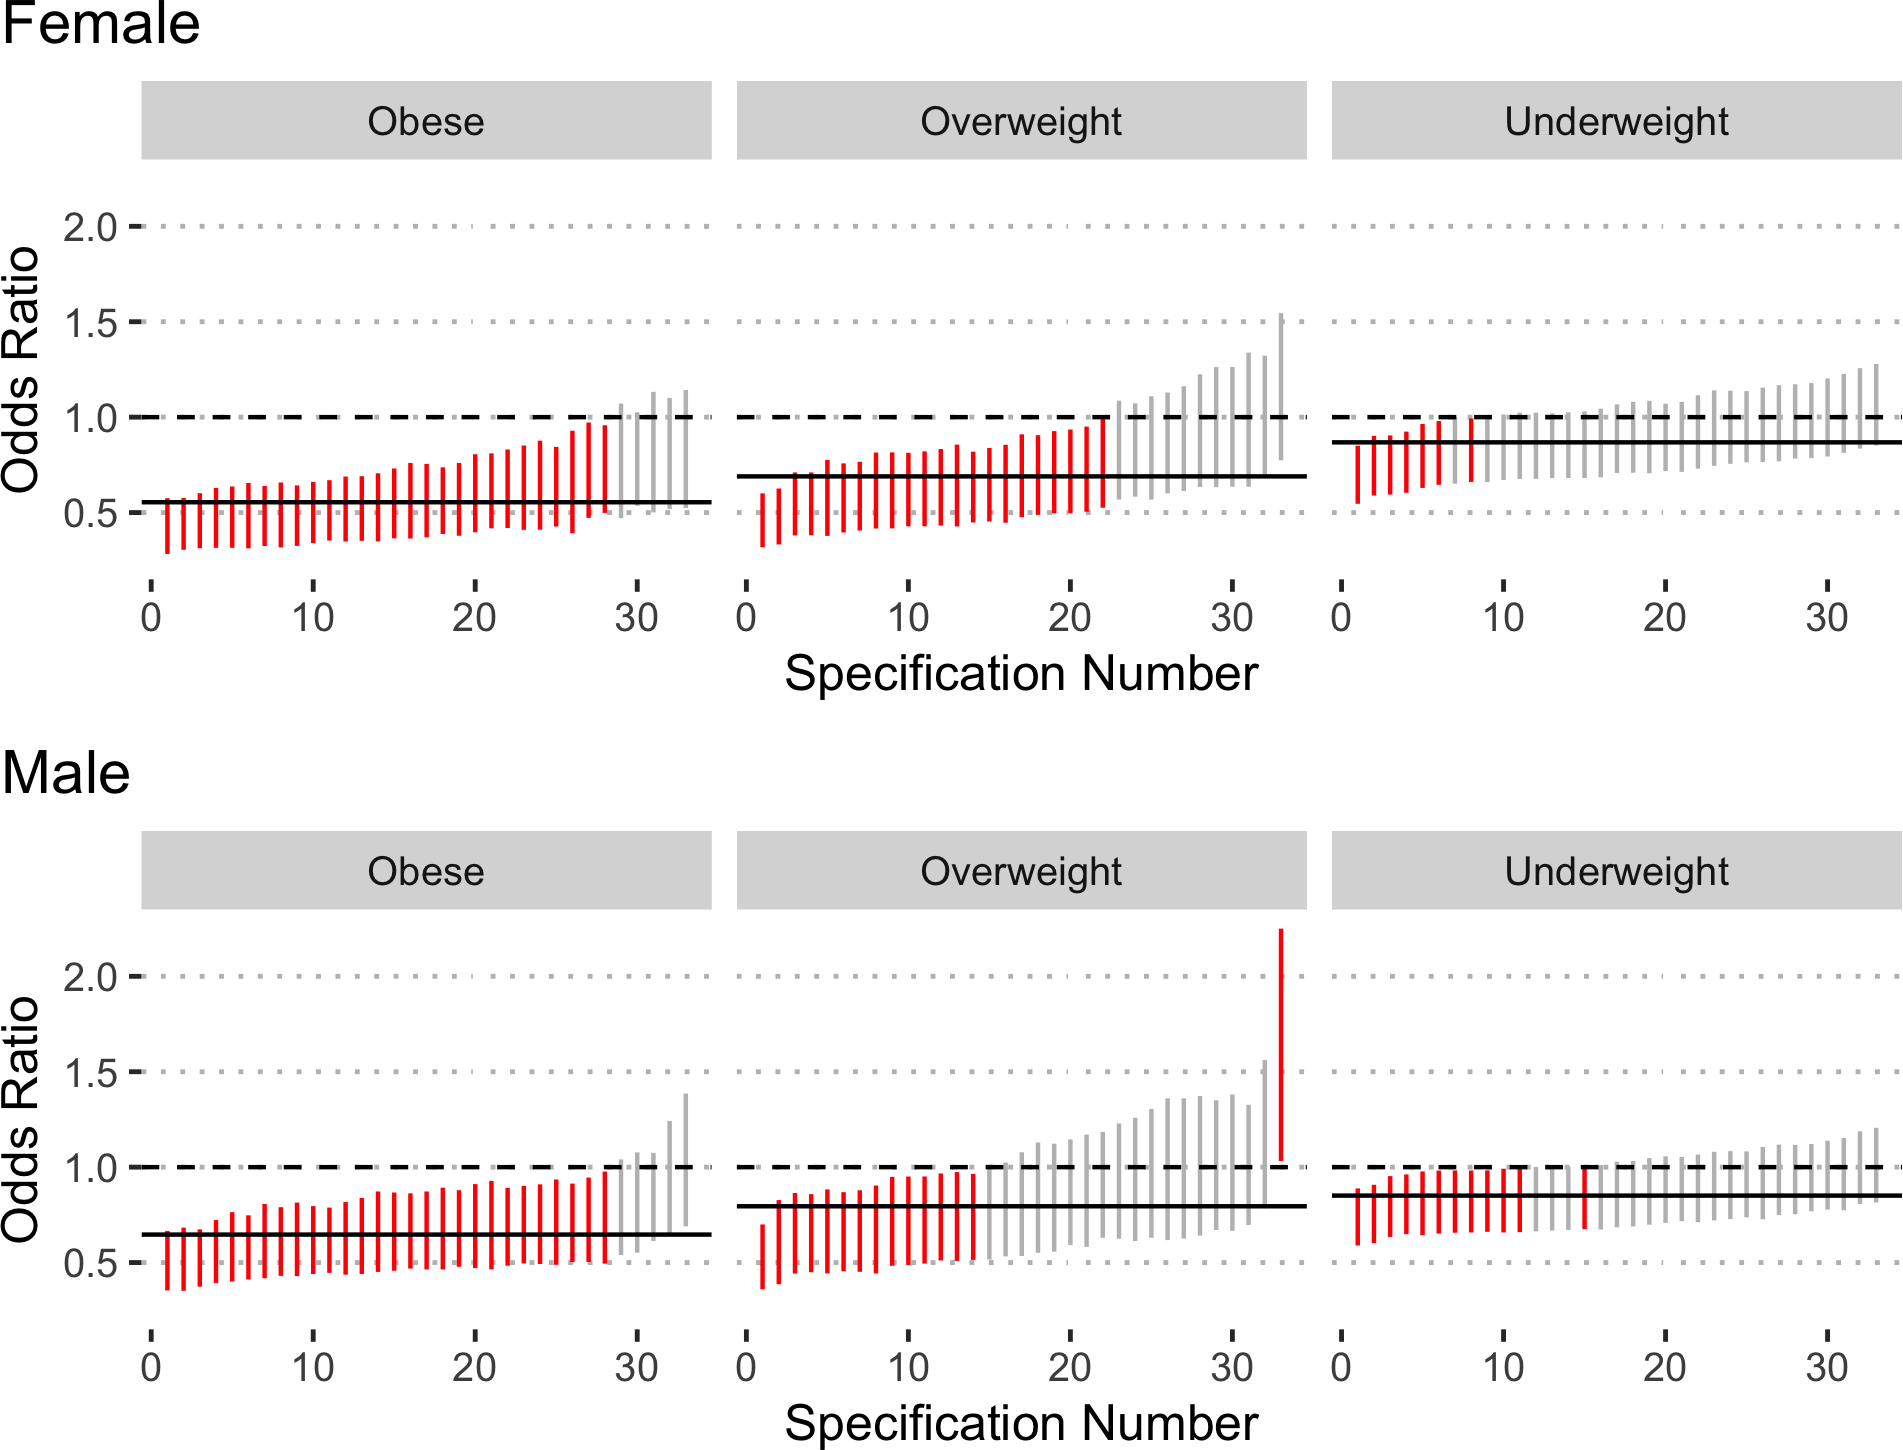
\includegraphics[height=5in]{bmi_personality_files/figure-latex/SESplot-1} \caption{ }\label{fig:SESplot}
\end{figure}

To test this question, we examine the estimates of the SES coefficient in the multinomial logistic models. These results are summarized in Figure \ref{fig:SESplot}. These figures display the odds ratios associated with the SES coefficient in each model; as a reminder, there are 33 models for each gender, each model regression the BMI category variable onto SES and one of the thirty-three individual difference measures. Figure @ref(fig:SES\_plot) represents the 95\% confidence interval around each estimate, for each non-reference category, with a vertical line. Lines are red if they do not contain 1 (the traditional null hypothesis, represented by the horizontal dashed line). A solid horizontal line represents the average coefficient estimate across all models. Models are ordered within weight comparison by size of the effect.

As evidenced by the figure, larger parental SES was consistently significantly associated with reduced odds of being obese among both boys and girls and reduced odds of being overweight among girls. SES was significantly associated with lower likelihood of being overweight among boys in 14 models, and lower likelihood of being underweight in only 7 and 12 models, for girls and boys, respectively. Overall, a one-standard deviation increase in parental SES was associated with being 45\% less likely to be obese and 31\% less likely to be overweight among girls, and with being 35\% less likely to be obese and 21\% less likely to be overweight among boys.

We note that the association between SES and weight categories tend to be somewhat sensitive to inclusion of personality traits, as coefficient estimates range from no affect on BMI to as much as half the likelihood.

\hypertarget{which-personality-traits-are-associated-with-bmi}{%
\subsubsection{Which personality traits are associated with BMI?}\label{which-personality-traits-are-associated-with-bmi}}

\begin{center}
\begin{ThreePartTable}
\small{
\begin{longtable}{lcccccc}\noalign{\getlongtablewidth\global\LTcapwidth=\longtablewidth}
\caption{\label{tab:tablepers}BMI category odds ratios associated with individual differences. All models control for parental SES. \* indicates p < .05}\\
\toprule
 & \multicolumn{3}{c}{Female} & \multicolumn{3}{c}{Male} \\
\cmidrule(r){2-4} \cmidrule(r){5-7}
Trait & Obese & Overweight & Underweight & Obese & Overweight & Underweight\\
\midrule
Cognitive Ability & 0.79 & 0.97 & 0.97 & 0.87 & 0.74* & 0.90\\
NA & [0.60, 1.04] & [0.76, 1.22] & [0.84, 1.12] & [0.68, 1.12] & [0.56, 0.98] & [0.78, 1.04]\\
Compassion & 0.99 & 1.02 & 1.12 & 0.96 & 0.95 & 1.04\\
NA & [0.76, 1.29] & [0.81, 1.29] & [0.96, 1.31] & [0.77, 1.20] & [0.73, 1.24] & [0.90, 1.21]\\
Irritability & 1.18 & 1.16 & 1.08 & 1.18 & 1.25 & 0.95\\
NA & [0.90, 1.55] & [0.89, 1.51] & [0.93, 1.25] & [0.92, 1.53] & [0.95, 1.65] & [0.82, 1.11]\\
Sociability & 0.75* & 0.78* & 0.66* & 0.87 & 0.83 & 0.78*\\
NA & [0.58, 0.98] & [0.62, 0.99] & [0.57, 0.76] & [0.68, 1.10] & [0.64, 1.08] & [0.67, 0.90]\\
Well Being & 0.52* & 0.53* & 0.62* & 0.81 & 1.02 & 0.75*\\
NA & [0.38, 0.70] & [0.40, 0.71] & [0.53, 0.72] & [0.62, 1.05] & [0.79, 1.32] & [0.65, 0.87]\\
Sensation Seeking & 1.03 & 1.13 & 1.11 & 0.83 & 1.25 & 0.74*\\
NA & [0.79, 1.35] & [0.89, 1.44] & [0.97, 1.28] & [0.63, 1.08] & [0.94, 1.65] & [0.63, 0.87]\\
Anxiety & 1.11 & 1.24 & 1.19* & 0.85 & 0.82 & 1.09\\
NA & [0.86, 1.44] & [0.96, 1.59] & [1.03, 1.37] & [0.65, 1.10] & [0.63, 1.07] & [0.94, 1.27]\\
Honesty & 0.72* & 0.79* & 0.94 & 0.98 & 0.96 & 0.98\\
NA & [0.56, 0.94] & [0.62, 0.99] & [0.80, 1.11] & [0.74, 1.28] & [0.74, 1.25] & [0.83, 1.15]\\
Industry & 0.71* & 0.88 & 0.76* & 0.94 & 0.94 & 0.92\\
NA & [0.54, 0.95] & [0.69, 1.13] & [0.65, 0.88] & [0.73, 1.23] & [0.71, 1.24] & [0.79, 1.07]\\
Intellect & 1.26 & 1.07 & 0.98 & 1.06 & 1.24 & 0.92\\
NA & [0.96, 1.67] & [0.84, 1.36] & [0.85, 1.13] & [0.79, 1.42] & [0.86, 1.80] & [0.78, 1.09]\\
Creativity & 0.94 & 0.99 & 1.07 & 0.95 & 1.06 & 1.03\\
NA & [0.72, 1.23] & [0.79, 1.24] & [0.92, 1.24] & [0.76, 1.19] & [0.79, 1.41] & [0.88, 1.19]\\
Impulsivity & 1.20 & 0.97 & 1.13 & 1.12 & 1.11 & 1.04\\
NA & [0.93, 1.55] & [0.76, 1.25] & [0.98, 1.31] & [0.88, 1.43] & [0.86, 1.43] & [0.89, 1.21]\\
Attention Seeking & 0.83 & 1.16 & 0.77* & 0.78* & 0.87 & 0.73*\\
NA & [0.63, 1.08] & [0.89, 1.51] & [0.67, 0.89] & [0.62, 0.99] & [0.66, 1.14] & [0.63, 0.85]\\
Order & 0.84 & 0.96 & 0.89 & 1.11 & 0.94 & 0.92\\
NA & [0.62, 1.14] & [0.75, 1.23] & [0.76, 1.04] & [0.86, 1.42] & [0.72, 1.22] & [0.79, 1.06]\\
Authoritarianism & 1.06 & 1.02 & 0.87 & 1.06 & 0.99 & 1.12\\
NA & [0.82, 1.37] & [0.80, 1.29] & [0.75, 1.01] & [0.81, 1.40] & [0.74, 1.32] & [0.96, 1.32]\\
Charisma & 1.02 & 0.93 & 0.84* & 0.87 & 1.28 & 0.79*\\
NA & [0.79, 1.31] & [0.73, 1.18] & [0.73, 0.97] & [0.67, 1.14] & [0.98, 1.68] & [0.68, 0.91]\\
Trust & 0.78 & 0.90 & 0.79* & 1.13 & 0.90 & 1.16\\
NA & [0.58, 1.05] & [0.72, 1.14] & [0.68, 0.92] & [0.87, 1.47] & [0.68, 1.20] & [0.99, 1.36]\\
Humor & 1.65* & 1.01 & 0.98 & 1.41* & 0.91 & 0.84*\\
NA & [1.14, 2.38] & [0.81, 1.27] & [0.85, 1.13] & [1.06, 1.88] & [0.69, 1.19] & [0.72, 0.98]\\
Emotional Expressiveness & 0.70* & 0.73* & 0.76* & 0.81 & 1.30 & 0.95\\
NA & [0.53, 0.92] & [0.57, 0.92] & [0.66, 0.87] & [0.63, 1.05] & [1.00, 1.69] & [0.82, 1.11]\\
Art Appreciation & 1.31 & 1.02 & 1.72* & 0.97 & 0.85 & 1.03\\
NA & [0.91, 1.89] & [0.81, 1.29] & [1.41, 2.09] & [0.75, 1.25] & [0.67, 1.08] & [0.88, 1.21]\\
Introspection & 1.06 & 0.85 & 1.25* & 1.03 & 0.87 & 0.94\\
NA & [0.81, 1.38] & [0.67, 1.07] & [1.07, 1.46] & [0.78, 1.36] & [0.68, 1.12] & [0.80, 1.09]\\
Perfectionism & 0.88 & 0.88 & 0.80* & 0.92 & 0.80 & 1.01\\
NA & [0.66, 1.18] & [0.69, 1.11] & [0.69, 0.92] & [0.72, 1.17] & [0.61, 1.05] & [0.86, 1.19]\\
Self Control & 0.49* & 1.14 & 1.07 & 0.81 & 0.83 & 1.00\\
NA & [0.35, 0.69] & [0.89, 1.46] & [0.92, 1.24] & [0.62, 1.06] & [0.65, 1.07] & [0.85, 1.17]\\
Conformity & 1.00 & 1.15 & 0.84* & 0.99 & 0.99 & 1.01\\
NA & [0.77, 1.29] & [0.91, 1.45] & [0.73, 0.97] & [0.76, 1.28] & [0.78, 1.26] & [0.86, 1.17]\\
Adaptability & 0.83 & 1.10 & 0.90 & 1.08 & 1.18 & 1.02\\
NA & [0.63, 1.09] & [0.87, 1.40] & [0.77, 1.04] & [0.82, 1.42] & [0.89, 1.55] & [0.88, 1.19]\\
Easy Goingness & 1.60* & 1.69* & 1.26* & 1.53* & 1.22 & 1.23*\\
NA & [1.17, 2.20] & [1.29, 2.21] & [1.08, 1.47] & [1.13, 2.07] & [0.94, 1.59] & [1.05, 1.43]\\
Emotional Stability & 0.80 & 0.89 & 0.75* & 1.10 & 1.11 & 0.87*\\
NA & [0.63, 1.02] & [0.70, 1.12] & [0.65, 0.86] & [0.84, 1.43] & [0.85, 1.45] & [0.75, 1.00]\\
Conservatism & 0.81 & 1.00 & 0.86* & 0.98 & 1.00 & 0.82*\\
NA & [0.61, 1.06] & [0.78, 1.28] & [0.74, 0.99] & [0.75, 1.27] & [0.77, 1.30] & [0.71, 0.96]\\
Agreeableness & 0.81 & 1.03 & 0.91 & 0.76* & 1.25 & 1.13\\
NA & [0.64, 1.04] & [0.81, 1.32] & [0.79, 1.06] & [0.60, 0.97] & [0.92, 1.68] & [0.96, 1.33]\\
Conscientiousness & 0.83 & 0.98 & 0.75* & 0.90 & 0.80 & 0.90\\
NA & [0.64, 1.09] & [0.76, 1.26] & [0.64, 0.88] & [0.68, 1.19] & [0.60, 1.06] & [0.77, 1.06]\\
Extraversion & 0.70* & 0.89 & 0.75* & 0.79 & 1.01 & 0.77*\\
NA & [0.54, 0.90] & [0.71, 1.13] & [0.65, 0.86] & [0.61, 1.03] & [0.76, 1.35] & [0.66, 0.89]\\
Neuroticism & 1.61* & 1.27 & 1.39* & 1.17 & 1.42* & 1.22*\\
NA & [1.20, 2.17] & [0.96, 1.68] & [1.20, 1.62] & [0.93, 1.49] & [1.08, 1.86] & [1.06, 1.41]\\
Openness & 1.06 & 1.04 & 1.24* & 1.22 & 0.92 & 0.92\\
NA & [0.81, 1.40] & [0.82, 1.33] & [1.07, 1.44] & [0.94, 1.57] & [0.69, 1.23] & [0.79, 1.08]\\
\bottomrule
\end{longtable}
}
\end{ThreePartTable}
\end{center}

\begin{figure}
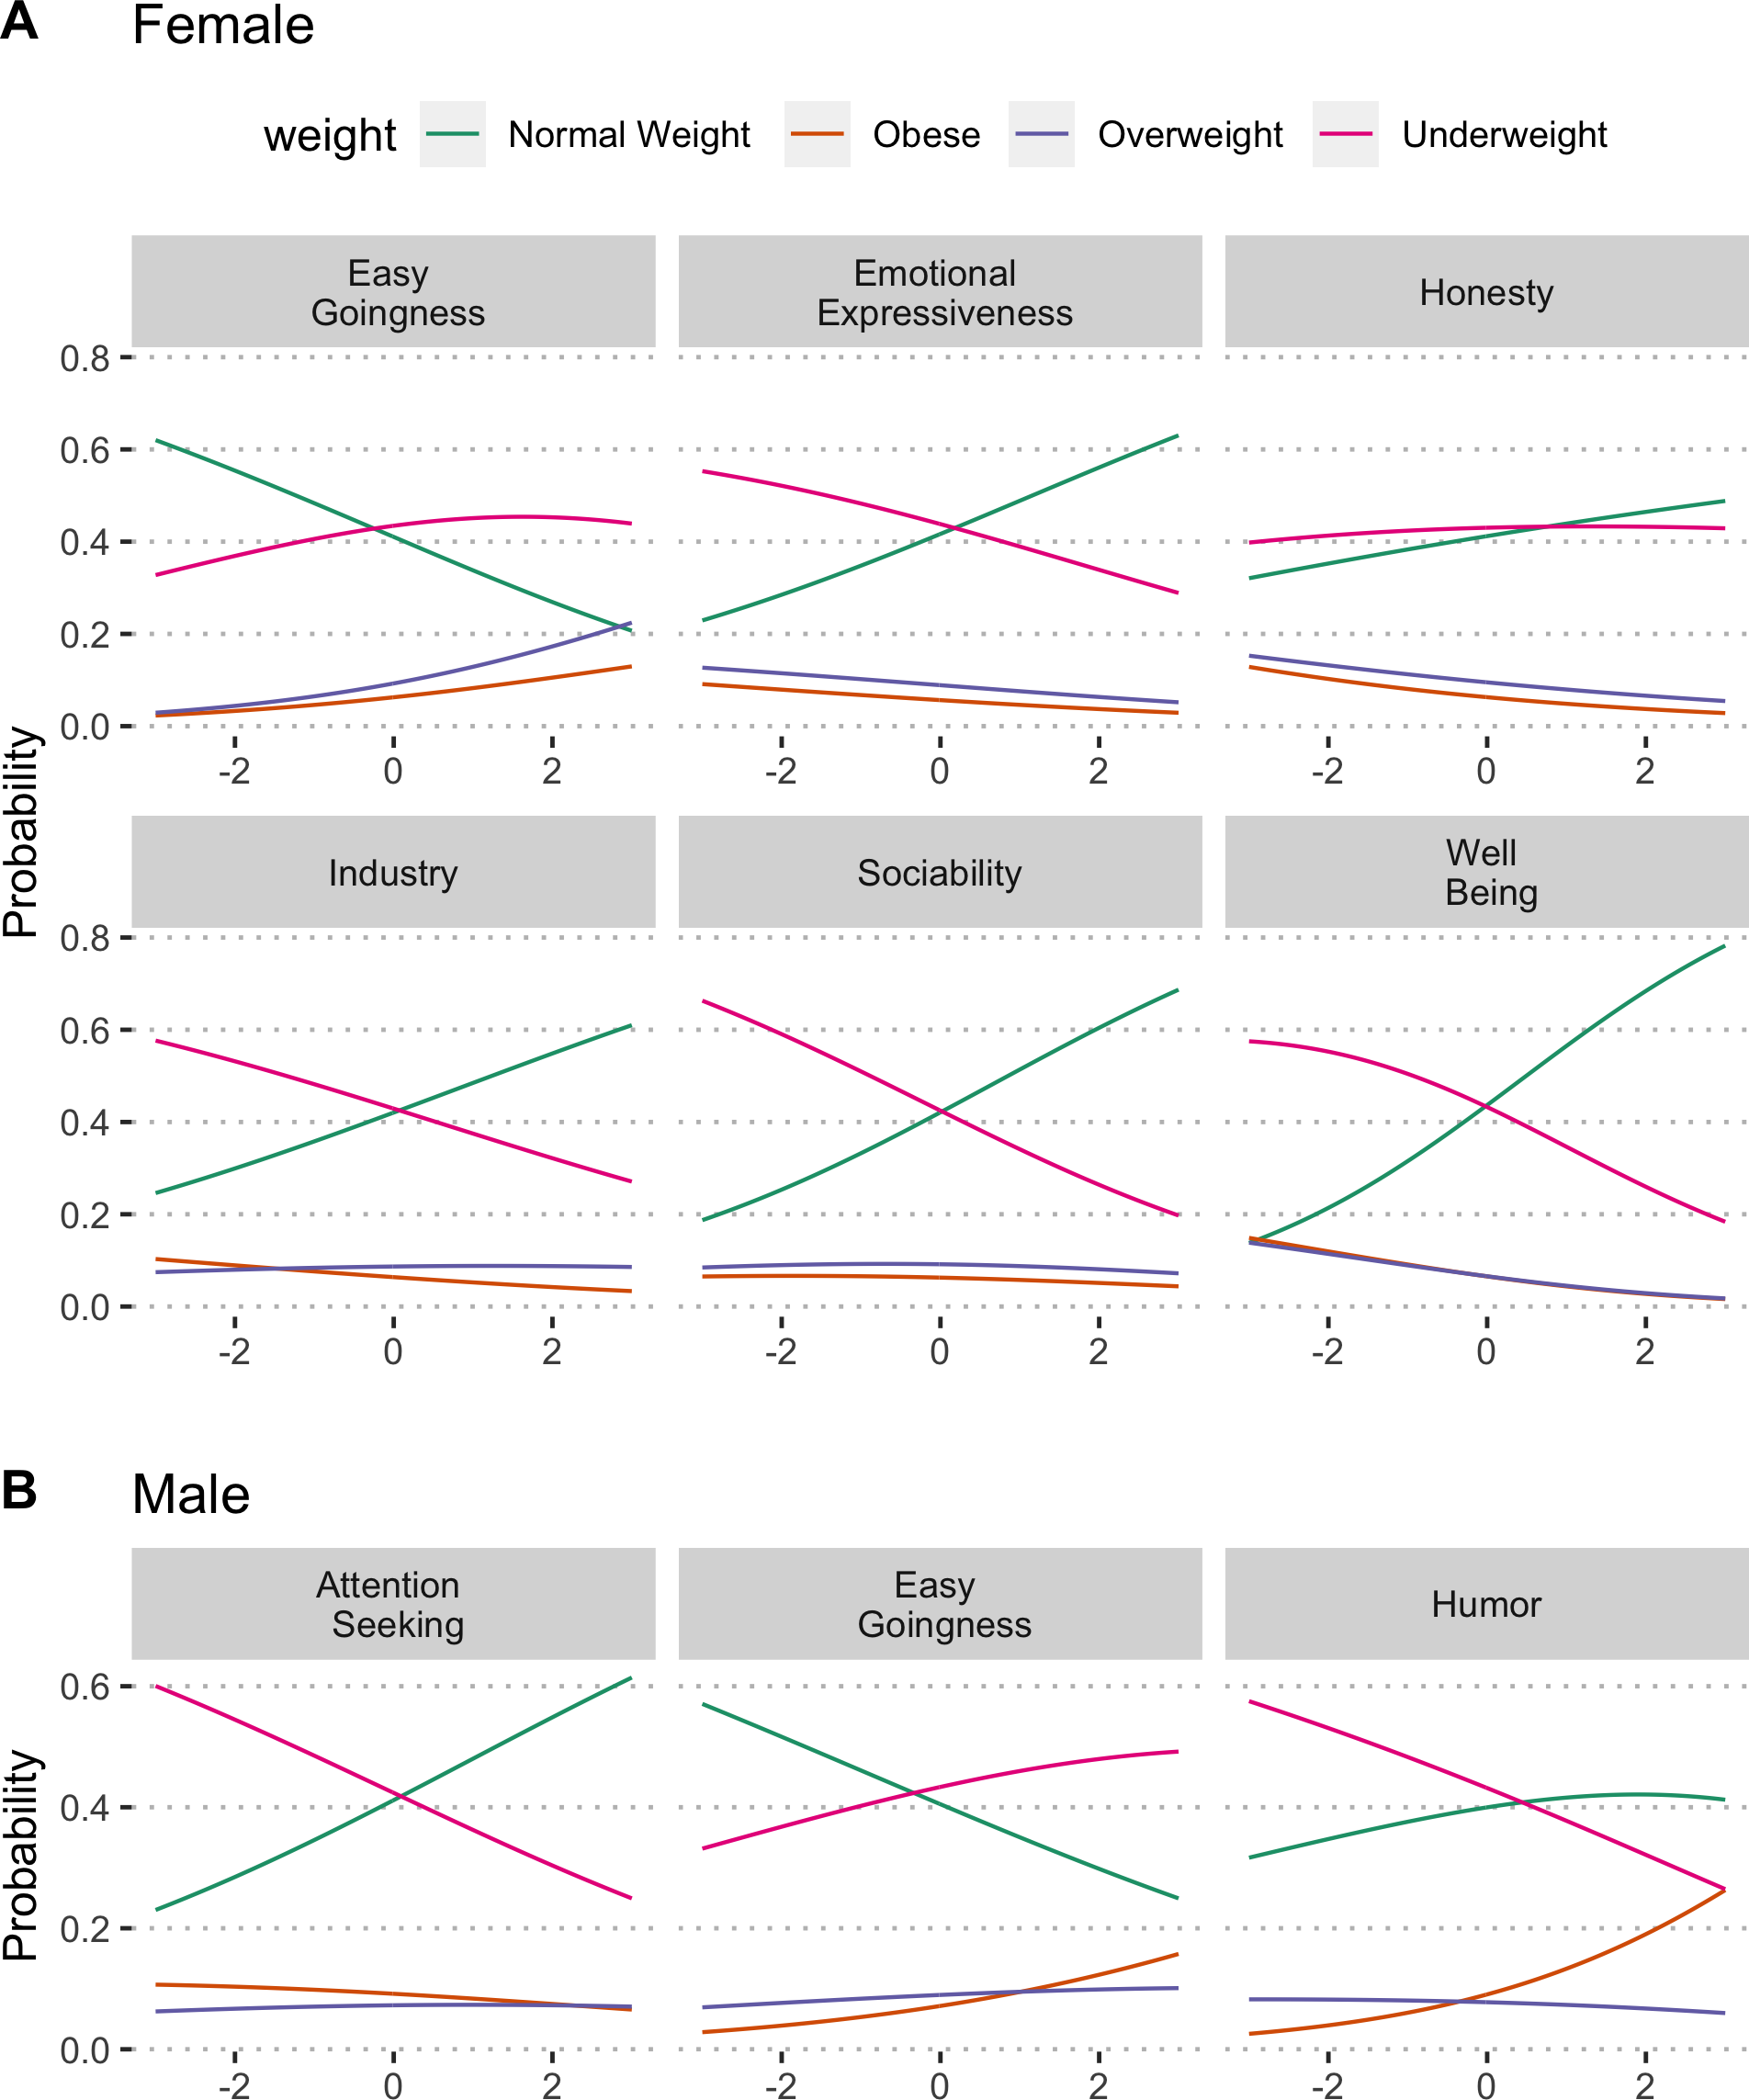
\includegraphics[height=8in]{bmi_personality_files/figure-latex/personplot-1} \caption{ }\label{fig:personplot}
\end{figure}

Next we examine the coefficients associated with personality traits -- here referring to cognitive ability, the Big Five, and the Narrow 27 -- in the models described above. All results are summarized in Table \ref{tab:tablepers}.

Two main patterns stand out. First, several traits were associated with both types of weight issues. More specifically, among adolescent girls, traits Sociability, Well-Being, and Emotional Expressiveness were significantly associated with reduced odds of all non-Normal categories. Trait Easy Goingness was significantly associated with increased of all non-Normal categories. In other words, adolescent girls low in Sociability, Well-Being and Emotional Expressiveness and high in Easy Goingness are at greater risk for both overweight/obesity and also underweight status. These associations are depicted in Figure @ref(fig:person\_plot)A. Furthermore, trait Honesty was associated with decreased risk of overweight and obese statuses; traits Extraversion, Neuroticism, and Industry were associated with decreased risk of obesity and underweight statuses.

For adolescent boys, far fewer traits were associated with weight category compared to for adolescent girls. Again, some traits were associated with both ends of the weight spectrum: Attention Seeking and Easy Goingnesss were associated with decreased and increased risk, respectively, of both obesity and being overweight. Trait Neuroticism was associated with increased risk of both being overweight and underweight, although not obese. Humor was associated with increased risk of being obese but decreased risk of being underweight, making this the only association in which an individual difference had a consistent ordinal relationship with weight. We note there was a gender difference in the number of traits significantly associated with BMI category; however, this difference is most likely a result of a larger sample of adolescent girls.

Of note, cognitive ability was largely unassociated with BMI category, with one exception: being associated with reduced risk for overweight compared to normal status among adolescent boys. This is surprising, given the extended literature on the relationship between cognitive ability and health.

The second pattern is that far more traits were significantly associated with (reduced or increased) risk for underweight, while relatively few traits were associated with risk for obesity or risk for being overweight. However, this pattern is most likely due to the relatively small sample of underweight adolescents in the study, compared to the other groups.

\hypertarget{does-the-relationship-of-personality-to-bmi-depend-on-ses}{%
\subsubsection{Does the relationship of personality to BMI depend on SES?}\label{does-the-relationship-of-personality-to-bmi-depend-on-ses}}

By adding an interaction term to each of our 33 models, we test the degree to which the relationship of personality to BMI category changes as a function of parental SES. As depicted in Figure \ref{fig:SESplot2}, the overwhelming finding was that the interaction terms were mainly non-significant. A handful of coefficients barely reach the statistical significance threshold, but this is expected due to chance alone.

\begin{figure}
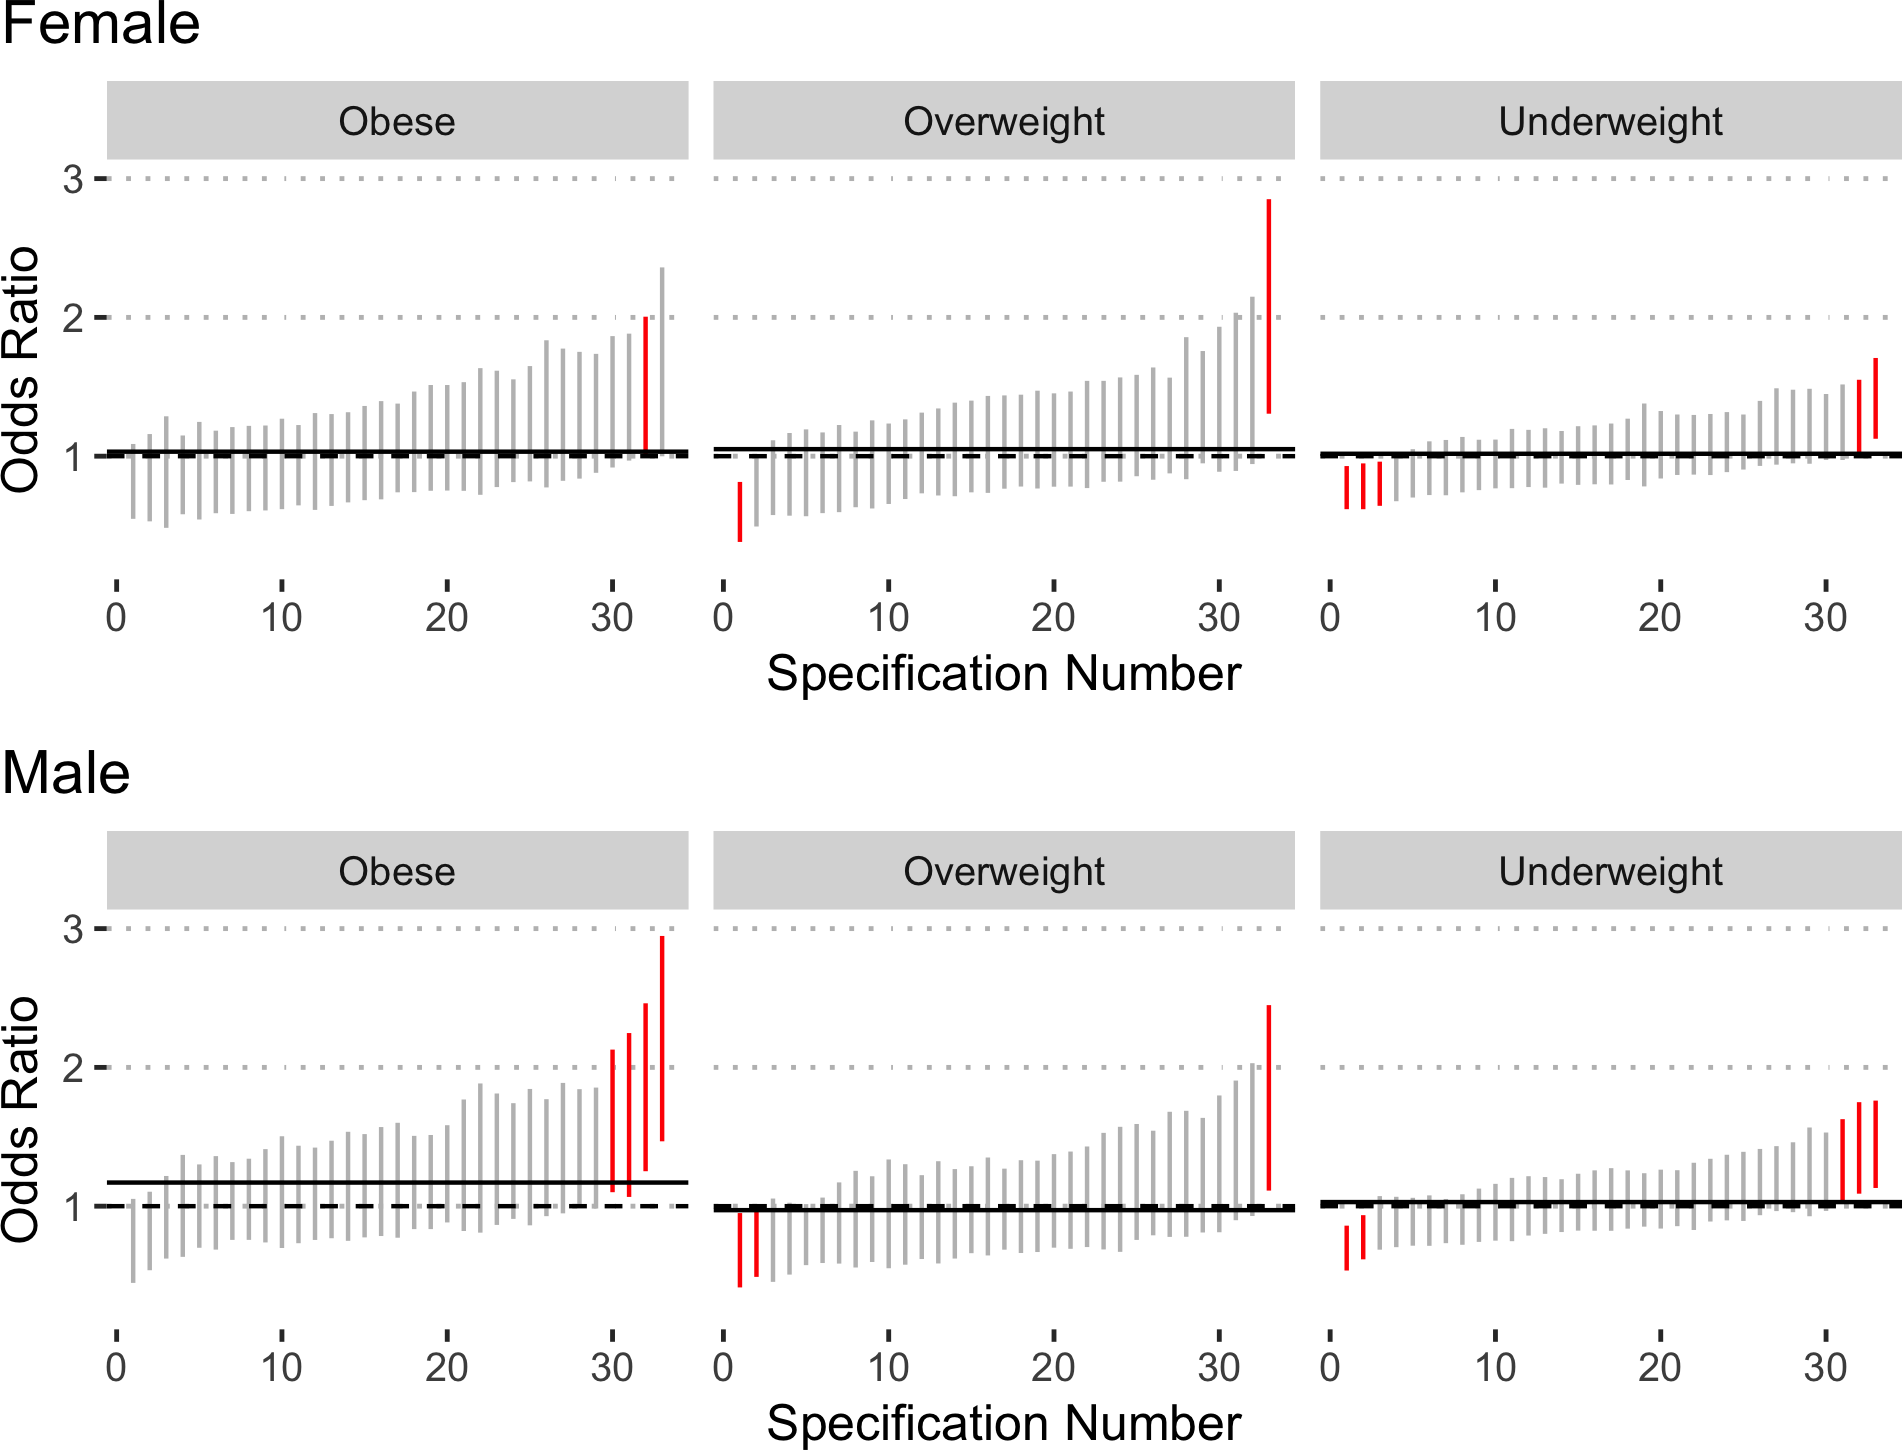
\includegraphics[height=5in]{bmi_personality_files/figure-latex/SESplot2-1} \caption{ }\label{fig:SESplot2}
\end{figure}

\hypertarget{sensitivity-analysis}{%
\paragraph{Sensitivity analysis}\label{sensitivity-analysis}}

After conducting our planned analyses, we were concerned that our results were potentially biased by the presence of data missing not at random. Specifically, we noticed that among our adolescent sample, approximately half did not report height or weight or both. The primary concern is that participants of specific BMIs may systematically skip questions about height or weight, leading to over or under estimates of in regression models.

To address this concern, we imputed missing height and weight values using 32 personality variables that were collected through our online data collection tool but were not used to estimate trait scores on any scales used in the study. These variables were chosen because there were enough pairwise administrations for each pair of variables that a principle components analysis including these variables and height and weight could converge. We used a single PCA imputation with regularization.

\begin{figure}
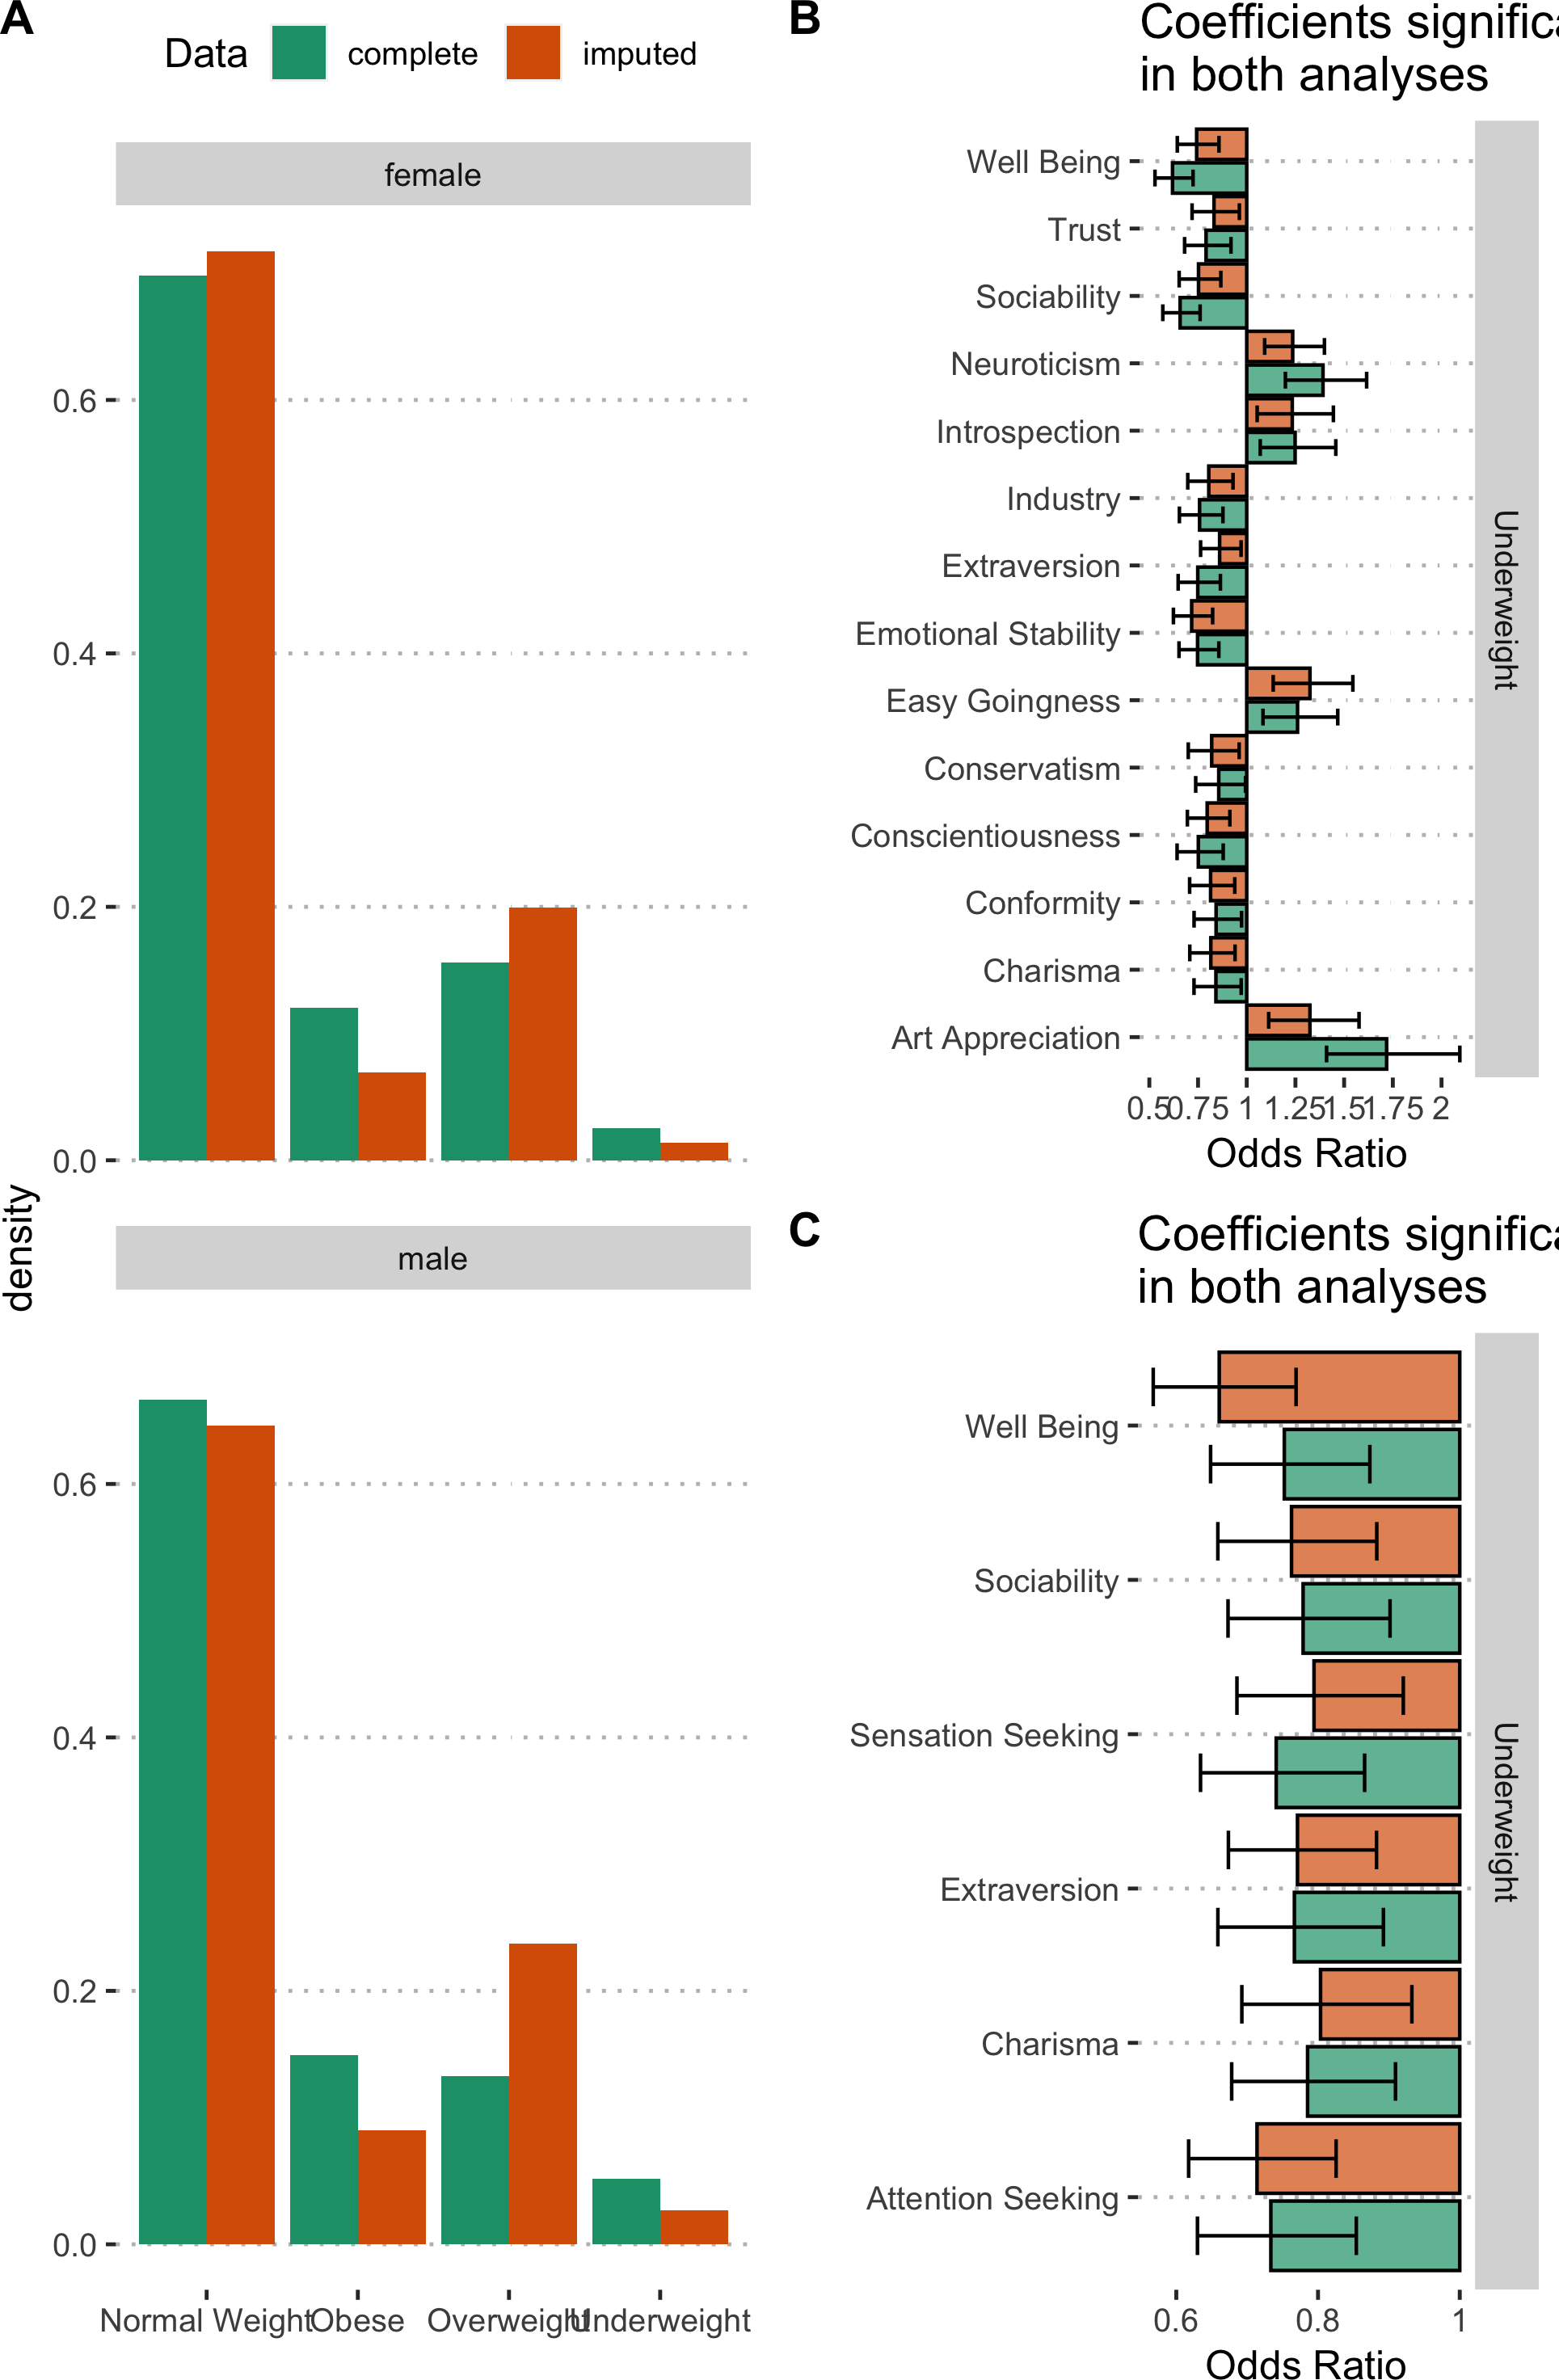
\includegraphics[height=10in]{bmi_personality_files/figure-latex/sens-1} \caption{ }\label{fig:sens}
\end{figure}

Imputation suggested that we were under-sampling from normal weight and overweight adolescents and oversampling obese and underweight adolescents (see Figure \ref{fig:sens}A). If imputed height and weight are included in the analyses, several key findings are no longer statistically significant. Of primary interest, the single association of cognitive ability with BMI category was no longer significant in these analyses.

However, some findings were robust to these sensitivity analyses. Interestingly, all were in the comparison of Underweight to Normal BMI category. These robust estimates are presented in Figure \ref{fig:sens}B and \ref{fig:sens}C. In sum, narrow traits of Well-Being

\hypertarget{how-does-personality-contribute-to-the-accuracy-of-bmi-prediction-models}{%
\subsubsection{How does personality contribute to the accuracy of BMI prediction models?}\label{how-does-personality-contribute-to-the-accuracy-of-bmi-prediction-models}}

Completion of the preregistered analyses yielded results that suggest that low parental SES is a robust risk factor for all non-normal BMI categories, that some personality traits play a role in non-normal weight for adolescents, and that the degree to which individual differences are associated with BMI does not depend on parental SES. However, one additional and unplanned question emerges from these analyses: to what extent does personality contribute predictive validity to estimates of BMI category and does that depend on the use of broad versus narrow traits?

To answer this question, we build three additional logistic regression models: BMI category regressed onto (1) parental SES, (2) parental SES plus all of the Big Five traits, and (3) parental SES plus all of the Narrow SPI 27. To avoid over-fitting, we used 10-fold cross-validation, repeated 10 times. The final model was selected using the summary metric of accuracy. These models were built using the same 75\% of the sample that was used in prior analyses. Finally, these model were used to predict BMI category in the hold-out sample (25\%), and these predictions were compared to reported BMI category for accuracy. Our accuracy metric is Area Under the Curve.

\begin{figure}
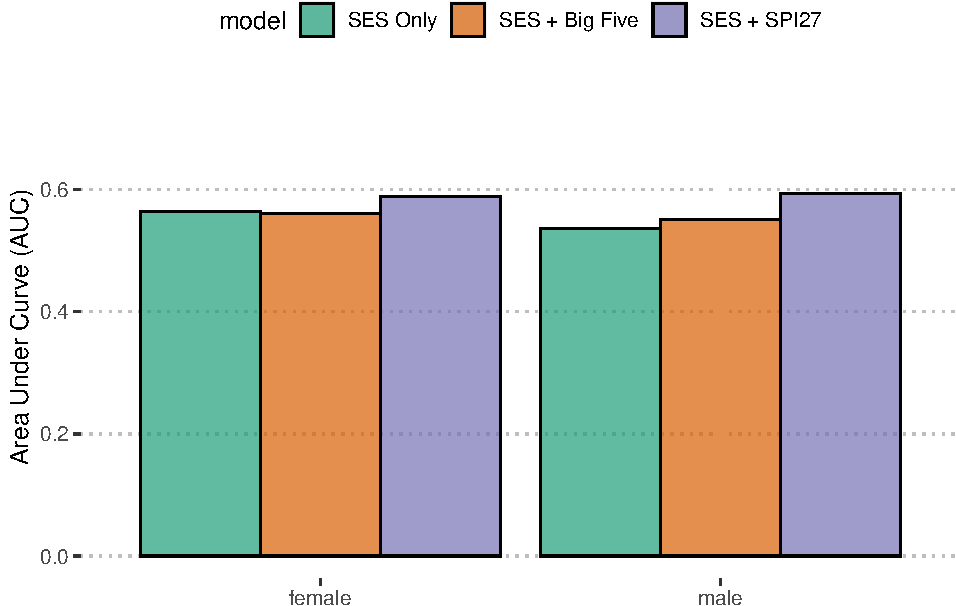
\includegraphics[width=5in]{bmi_personality_files/figure-latex/auc-1} \caption{ }\label{fig:auc}
\end{figure}

Results are summarized in Figure \ref{fig:auc}. Models including SES plus personality did as well or better than models with SES only \((AUC_{female} = 0.56, AUC_{male} = 0.54)\). The models using the set of narrow SPI traits \((AUC_{female} = 0.59, AUC_{male} = 0.59)\) added more predictive power than models using the Big Five \((AUC_{female} = 0.56, AUC_{male} = 0.55)\). However, the gain in predictive power was modest, improving estimates by about 10\%.

\hypertarget{discussion}{%
\section{Discussion}\label{discussion}}

The current study included many analyses, providing a wealth of potential conclusions. We discuss our interpretations starting with the conclusions we are most confident in and working towards conclusions that have less evidentiary value.

First, we begin with the conclusions we have strong confidence in. We believe it is undisputable at this point that higher parental socioeconomic status (SES) is associated with lower risk of adolescent girls and boys being underweight, overweight, and obese, implying that SES may be protective against weight problems on both ends of the spectrum. This finding was robust to the inclusion of nearly all traits, and conforms with prior findings in the literature.

In addition, we conclude that some personality traits are independently associated risk for being underweight, compared to normal, even accoutning for parental SES. We are especially confident in the associations between trait neuroticism and the highly associated narrow traits well-being and emotional stability among adolescent girls, and the well-being, sensation seeking, and attention seeking among adolesecnt boys.

Next, there is some evidence that personality traits may also be independently associated with risk for being overweight or obese. We have reduced confidence in these findings given that these associations were sensitive to the imputation of missing data in our study.

\hypertarget{findings-in-context-research}{%
\subsection{Findings in context -- research}\label{findings-in-context-research}}

It is notable that many teens were unwilling (or perhaps unable) to provide their height and/or weight on an anonymous self-report assessment of personality. Body size is scrutinized among adolescents and, for some individuals, may be stimatized by their peers, so it is unsuprirising that at least some individuals chose not to report these values. However roughly half of our sample of US adolescents skipped one or both of these questions, suggesting large bias in self-report studies attempting to measure these variables. All studies of BMI in adolescents must take great care to attend to missigness in data and, ideally, avoid the use of self-report as the primary means by which these data are colleted.

It should be noted that associations between SES and personality are likely bidirectional. Certainly across the lifespan, there is strong evidence of the effects of personality on socioeconomic status in adulthood (Barrick \& Mount, 1991; Duckworth, Weir, Tsukayama, \& Kwok, 2012; Wilcox, Block, \& Eisenstein, 2011). This suggests that some of the direct effects of personality or SES on weight are obscured by controlling for the other; indeed, the range of coefficients for SES across models implies that the choice of trait covariate may have substantial impact on the conclusions drawn in a particular study.

\hypertarget{limitations}{%
\subsection{Limitations}\label{limitations}}

The primary limitations of the current study are the use of self-reported height and weight, which imposes bias through inaccuracy and missingness, and self-selection into the study. Regarding the former, several results were robust to sensitivity analysis, including the effect of parental socioeconomic status, the lack of interaction effects, and many relationships between personality traits and risk for being underweight compared to normal.Regarding self-selection, however, we are somewhat limited in our ability to test the boundaries of our effects. We note here that broadly, people who voluntarily visit this website represent a broad range of ethnic backgrounds and geographic locations, although it tends to skew more educated than the general population in adult samples (citation masked).

\hypertarget{conclusion}{%
\section{Conclusion}\label{conclusion}}

\newpage

\hypertarget{references}{%
\section{References}\label{references}}

\begingroup
\setlength{\parindent}{-0.5in}
\setlength{\leftskip}{0.5in}

\hypertarget{refs}{}
\leavevmode\hypertarget{ref-ayer2011adolescent}{}%
Ayer, L., Rettew, D., Althoff, R. R., Willemsen, G., Ligthart, L., Hudziak, J. J., \& Boomsma, D. I. (2011). Adolescent personality profiles, neighborhood income, and young adult alcohol use: A longitudinal study. \emph{Addictive Behaviors}, \emph{36}(12), 1301--1304.

\leavevmode\hypertarget{ref-barefoot1991hostility}{}%
Barefoot, J. C., Peterson, B. L., Dahlstrom, W. G., Siegler, I. C., Anderson, N. B., \& Williams Jr, R. B. (1991). Hostility patterns and health implications: Correlates of cook-medley hostility scale scores in a national survey. \emph{Health Psychology}, \emph{10}(1), 18.

\leavevmode\hypertarget{ref-barrick1991big}{}%
Barrick, M. R., \& Mount, M. K. (1991). The big five personality dimensions and job performance: A meta-analysis. \emph{Personnel Psychology}, \emph{44}(1), 1--26.

\leavevmode\hypertarget{ref-bogg2004conscientiousness}{}%
Bogg, T., \& Roberts, B. W. (2004). Conscientiousness and health-related behaviors: A meta-analysis of the leading behavioral contributors to mortality. \emph{Psychological Bulletin}, \emph{130}(6), 887.

\leavevmode\hypertarget{ref-bosma1999social}{}%
Bosma, H., Mheen, H. D. van de, \& Mackenbach, J. P. (1999). Social class in childhood and general health in adulthood: Questionnaire study of contribution of psychological attributes. \emph{Bmj}, \emph{318}(7175), 18--22.

\leavevmode\hypertarget{ref-condon2018sapa}{}%
Condon, D. M. (2018). The sapa personality inventory: An empirically-derived, hierarchically-organized self-report personality assessment model.

\leavevmode\hypertarget{ref-conger2007interactionist}{}%
Conger, R. D., \& Donnellan, M. B. (2007). An interactionist perspective on the socioeconomic context of human development. \emph{Annu. Rev. Psychol.}, \emph{58}, 175--199.

\leavevmode\hypertarget{ref-cooper2009strong}{}%
Cooper, W. H., \& Withey, M. J. (2009). The strong situation hypothesis. \emph{Personality and Social Psychology Review}, \emph{13}(1), 62--72.

\leavevmode\hypertarget{ref-cournot2006relation}{}%
Cournot, M., Marquie, J., Ansiau, D., Martinaud, C., Fonds, H., Ferrieres, J., \& Ruidavets, J. (2006). Relation between body mass index and cognitive function in healthy middle-aged men and women. \emph{Neurology}, \emph{67}(7), 1208--1214.

\leavevmode\hypertarget{ref-deckers2015does}{}%
Deckers, T., Falk, A., Kosse, F., \& Schildberg-Hörisch, H. (2015). How does socio-economic status shape a child's personality?

\leavevmode\hypertarget{ref-delaney2012socioeconomic}{}%
Delaney, L., \& Doyle, O. (2012). Socioeconomic differences in early childhood time preferences. \emph{Journal of Economic Psychology}, \emph{33}(1), 237--247.

\leavevmode\hypertarget{ref-centers2000cdc}{}%
Disease Control, C. for, Prevention, \& others. (2000). CDC growth charts for the united states: Methods and development. \emph{Vital and Health Statistics}, \emph{11}(246), 1--190.

\leavevmode\hypertarget{ref-drenowatz2010influence}{}%
Drenowatz, C., Eisenmann, J. C., Pfeiffer, K. A., Welk, G., Heelan, K., Gentile, D., \& Walsh, D. (2010). Influence of socio-economic status on habitual physical activity and sedentary behavior in 8-to 11-year old children. \emph{BMC Public Health}, \emph{10}(1), 214.

\leavevmode\hypertarget{ref-duckworth2012does}{}%
Duckworth, A. L., Weir, D. R., Tsukayama, E., \& Kwok, D. (2012). Who does well in life? Conscientious adults excel in both objective and subjective success. \emph{Frontiers in Psychology}, \emph{3}, 356.

\leavevmode\hypertarget{ref-fokeena2012there}{}%
Fokeena, W. B., \& Jeewon, R. (2012). Is there an association between socioeconomic status and body mass index among adolescents in mauritius? \emph{The Scientific World Journal}, \emph{2012}.

\leavevmode\hypertarget{ref-frieden2010reducing}{}%
Frieden, T. R., Dietz, W., \& Collins, J. (2010). Reducing childhood obesity through policy change: Acting now to prevent obesity. \emph{Health Affairs}, \emph{29}(3), 357--363.

\leavevmode\hypertarget{ref-hampson2007mechanisms}{}%
Hampson, S. E., Goldberg, L. R., Vogt, T. M., \& Dubanoski, J. P. (2007). Mechanisms by which childhood personality traits influence adult health status: Educational attainment and healthy behaviors. \emph{Health Psychology}, \emph{26}(1), 121.

\leavevmode\hypertarget{ref-haworth2010heritability}{}%
Haworth, C. M., Wright, M. J., Luciano, M., Martin, N. G., Geus, E. J. de, Beijsterveldt, C. E. van, \ldots{} others. (2010). The heritability of general cognitive ability increases linearly from childhood to young adulthood. \emph{Molecular Psychiatry}, \emph{15}(11), 1112.

\leavevmode\hypertarget{ref-us2014healthy}{}%
Healthy People. (2014). Healthy people 2020. Washington, dc. \emph{US Department of Health and Human Services and Office of Disease Prevention and Health Promotion}.

\leavevmode\hypertarget{ref-kakizaki2008personality}{}%
Kakizaki, M., Kuriyama, S., Sato, Y., Shimazu, T., Matsuda-Ohmori, K., Nakaya, N., \ldots{} Tsuji, I. (2008). Personality and body mass index: A cross-sectional analysis from the miyagi cohort study. \emph{Journal of Psychosomatic Research}, \emph{64}(1), 71--80.

\leavevmode\hypertarget{ref-korner2003influence}{}%
Körner, A., Geyer, M., Gunzelmann, T., \& Brähler, E. (2003). The influence of socio-demographic factors on personality dimensions in the elderly. \emph{Zeitschrift Fur Gerontologie Und Geriatrie}, \emph{36}(2), 130--137.

\leavevmode\hypertarget{ref-liang2014neurocognitive}{}%
Liang, J., Matheson, B., Kaye, W., \& Boutelle, K. (2014). Neurocognitive correlates of obesity and obesity-related behaviors in children and adolescents. \emph{International Journal of Obesity}, \emph{38}(4), 494.

\leavevmode\hypertarget{ref-lipina2005performance}{}%
Lipina, S. J., Martelli, M. I., Vuelta, B., \& Colombo, J. A. (2005). Performance on the a-not-b task of argentinean infants from unsatisfied and satisfied basic needs homes. \emph{Interamerican Journal of Psychology}, \emph{39}(1), 49--60.

\leavevmode\hypertarget{ref-lohman2006associations}{}%
Lohman, T. G., Ring, K., Schmitz, K. H., Treuth, M. S., Loftin, M., Yang, S., \ldots{} Going, S. (2006). Associations of body size and composition with physical activity in adolescent girls. \emph{Medicine and Science in Sports and Exercise}, \emph{38}(6), 1175.

\leavevmode\hypertarget{ref-lynam2000interaction}{}%
Lynam, D. R., Caspi, A., Moffit, T. E., Wikström, P.-O., Loeber, R., \& Novak, S. (2000). The interaction between impulsivity and neighborhood context on offending: The effects of impulsivity are stronger in poorer neighborhoods. \emph{Journal of Abnormal Psychology}, \emph{109}(4), 563.

\leavevmode\hypertarget{ref-merikangas2010prevalence}{}%
Merikangas, K. R., He, J.-P., Brody, D., Fisher, P. W., Bourdon, K., \& Koretz, D. S. (2010). Prevalence and treatment of mental disorders among us children in the 2001--2004 nhanes. \emph{Pediatrics}, \emph{125}(1), 75--81.

\leavevmode\hypertarget{ref-molnar2004unsafe}{}%
Molnar, B. E., Gortmaker, S. L., Bull, F. C., \& Buka, S. L. (2004). Unsafe to play? Neighborhood disorder and lack of safety predict reduced physical activity among urban children and adolescents. \emph{American Journal of Health Promotion}, \emph{18}(5), 378--386.

\leavevmode\hypertarget{ref-mond2007associations}{}%
Mond, J., Stich, H., Hay, P., Krämer, A., \& Baune, B. (2007). Associations between obesity and developmental functioning in pre-school children: A population-based study. \emph{International Journal of Obesity}, \emph{31}(7), 1068.

\leavevmode\hypertarget{ref-o2006socio}{}%
O'Dea, J. A., \& Wilson, R. (2006). Socio-cognitive and nutritional factors associated with body mass index in children and adolescents: Possibilities for childhood obesity prevention. \emph{Health Education Research}, \emph{21}(6), 796--805.

\leavevmode\hypertarget{ref-ogden2014prevalence}{}%
Ogden, C. L., Carroll, M. D., Kit, B. K., \& Flegal, K. M. (2014). Prevalence of childhood and adult obesity in the united states, 2011-2012. \emph{Jama}, \emph{311}(8), 806--814.

\leavevmode\hypertarget{ref-provencher2008personality}{}%
Provencher, V., Bégin, C., Gagnon-Girouard, M.-P., Tremblay, A., Boivin, S., \& Lemieux, S. (2008). Personality traits in overweight and obese women: Associations with bmi and eating behaviors. \emph{Eating Behaviors}, \emph{9}(3), 294--302.

\leavevmode\hypertarget{ref-rhodes2006personality}{}%
Rhodes, R., \& Smith, N. (2006). Personality correlates of physical activity: A review and meta-analysis. \emph{British Journal of Sports Medicine}, \emph{40}(12), 958--965.

\leavevmode\hypertarget{ref-sabia2008body}{}%
Sabia, S., Kivimaki, M., Shipley, M. J., Marmot, M. G., \& Singh-Manoux, A. (2008). Body mass index over the adult life course and cognition in late midlife: The whitehall ii cohort study. \emph{The American Journal of Clinical Nutrition}, \emph{89}(2), 601--607.

\leavevmode\hypertarget{ref-shanahan2014conscientiousness}{}%
Shanahan, M. J., Hill, P. L., Roberts, B. W., Eccles, J., \& Friedman, H. S. (2014). Conscientiousness, health, and aging: The life course of personality model. \emph{Developmental Psychology}, \emph{50}(5), 1407.

\leavevmode\hypertarget{ref-neumarkeffect}{}%
Sherwood, N. E., Wall, M., Neumark-Sztainer, D., \& Story, M. (2009). Effect of socioeconomic status on weight change patterns in adolescents. \emph{Preventing Chronic Disease}, \emph{6}(1).

\leavevmode\hypertarget{ref-shrewsbury2008socioeconomic}{}%
Shrewsbury, V., \& Wardle, J. (2008). Socioeconomic status and adiposity in childhood: A systematic review of cross-sectional studies 1990--2005. \emph{Obesity}, \emph{16}(2), 275--284.

\leavevmode\hypertarget{ref-siervogel2003puberty}{}%
Siervogel, R. M., Demerath, E. W., Schubert, C., Remsberg, K. E., Chumlea, W. C., Sun, S., \ldots{} Towne, B. (2003). Puberty and body composition. \emph{Hormone Research in Paediatrics}, \emph{60}(Suppl. 1), 36--45.

\leavevmode\hypertarget{ref-smith1992public}{}%
Smith, A. M., \& Baghurst, K. I. (1992). Public health implications of dietary differences between social status and occupational category groups. \emph{Journal of Epidemiology \& Community Health}, \emph{46}(4), 409--416.

\leavevmode\hypertarget{ref-striegel1986toward}{}%
Striegel-Moore, R. H., Silberstein, L. R., \& Rodin, J. (1986). Toward an understanding of risk factors for bulimia. \emph{American Psychologist}, \emph{41}(3), 246.

\leavevmode\hypertarget{ref-sutin2011personality}{}%
Sutin, A. R., Ferrucci, L., Zonderman, A. B., \& Terracciano, A. (2011). Personality and obesity across the adult life span. \emph{Journal of Personality and Social Psychology}, \emph{101}(3), 579.

\leavevmode\hypertarget{ref-sutin2015personality}{}%
Sutin, A. R., Stephan, Y., Wang, L., Gao, S., Wang, P., \& Terracciano, A. (2015). Personality traits and body mass index in asian populations. \emph{Journal of Research in Personality}, \emph{58}, 137--142.

\leavevmode\hypertarget{ref-terracciano2009facets}{}%
Terracciano, A., Sutin, A. R., McCrae, R. R., Deiana, B., Ferrucci, L., Schlessinger, D., \ldots{} Costa Jr, P. T. (2009). Facets of personality linked to underweight and overweight. \emph{Psychosomatic Medicine}, \emph{71}(6), 682.

\leavevmode\hypertarget{ref-tuvblad2006heritability}{}%
Tuvblad, C., Grann, M., \& Lichtenstein, P. (2006). Heritability for adolescent antisocial behavior differs with socioeconomic status: Gene--environment interaction. \emph{Journal of Child Psychology and Psychiatry}, \emph{47}(7), 734--743.

\leavevmode\hypertarget{ref-wagerman2009personality}{}%
Wagerman, S. A., \& Funder, D. C. (2009). Personality psychology of situations.

\leavevmode\hypertarget{ref-wang2007}{}%
Wang, Y., Liang, L., Tussing, C., Braunschweig, C., Caballero B, \& Flay, B. (2007). Obesity and related risk factors among low socio-economic status minority students in chicago. \emph{Public Health Nutrition}, \emph{10}(9), 927--938.

\leavevmode\hypertarget{ref-wilcox2011leave}{}%
Wilcox, K., Block, L. G., \& Eisenstein, E. M. (2011). Leave home without it? The effects of credit card debt and available credit on spending. \emph{Journal of Marketing Research}, \emph{48}(SPL), S78--S90.

\leavevmode\hypertarget{ref-ayer2011adolescent}{}%
Ayer, L., Rettew, D., Althoff, R. R., Willemsen, G., Ligthart, L., Hudziak, J. J., \& Boomsma, D. I. (2011). Adolescent personality profiles, neighborhood income, and young adult alcohol use: A longitudinal study. \emph{Addictive Behaviors}, \emph{36}(12), 1301--1304.

\leavevmode\hypertarget{ref-barefoot1991hostility}{}%
Barefoot, J. C., Peterson, B. L., Dahlstrom, W. G., Siegler, I. C., Anderson, N. B., \& Williams Jr, R. B. (1991). Hostility patterns and health implications: Correlates of cook-medley hostility scale scores in a national survey. \emph{Health Psychology}, \emph{10}(1), 18.

\leavevmode\hypertarget{ref-barrick1991big}{}%
Barrick, M. R., \& Mount, M. K. (1991). The big five personality dimensions and job performance: A meta-analysis. \emph{Personnel Psychology}, \emph{44}(1), 1--26.

\leavevmode\hypertarget{ref-bogg2004conscientiousness}{}%
Bogg, T., \& Roberts, B. W. (2004). Conscientiousness and health-related behaviors: A meta-analysis of the leading behavioral contributors to mortality. \emph{Psychological Bulletin}, \emph{130}(6), 887.

\leavevmode\hypertarget{ref-bosma1999social}{}%
Bosma, H., Mheen, H. D. van de, \& Mackenbach, J. P. (1999). Social class in childhood and general health in adulthood: Questionnaire study of contribution of psychological attributes. \emph{Bmj}, \emph{318}(7175), 18--22.

\leavevmode\hypertarget{ref-condon2018sapa}{}%
Condon, D. M. (2018). The sapa personality inventory: An empirically-derived, hierarchically-organized self-report personality assessment model.

\leavevmode\hypertarget{ref-conger2007interactionist}{}%
Conger, R. D., \& Donnellan, M. B. (2007). An interactionist perspective on the socioeconomic context of human development. \emph{Annu. Rev. Psychol.}, \emph{58}, 175--199.

\leavevmode\hypertarget{ref-cooper2009strong}{}%
Cooper, W. H., \& Withey, M. J. (2009). The strong situation hypothesis. \emph{Personality and Social Psychology Review}, \emph{13}(1), 62--72.

\leavevmode\hypertarget{ref-cournot2006relation}{}%
Cournot, M., Marquie, J., Ansiau, D., Martinaud, C., Fonds, H., Ferrieres, J., \& Ruidavets, J. (2006). Relation between body mass index and cognitive function in healthy middle-aged men and women. \emph{Neurology}, \emph{67}(7), 1208--1214.

\leavevmode\hypertarget{ref-deckers2015does}{}%
Deckers, T., Falk, A., Kosse, F., \& Schildberg-Hörisch, H. (2015). How does socio-economic status shape a child's personality?

\leavevmode\hypertarget{ref-delaney2012socioeconomic}{}%
Delaney, L., \& Doyle, O. (2012). Socioeconomic differences in early childhood time preferences. \emph{Journal of Economic Psychology}, \emph{33}(1), 237--247.

\leavevmode\hypertarget{ref-centers2000cdc}{}%
Disease Control, C. for, Prevention, \& others. (2000). CDC growth charts for the united states: Methods and development. \emph{Vital and Health Statistics}, \emph{11}(246), 1--190.

\leavevmode\hypertarget{ref-drenowatz2010influence}{}%
Drenowatz, C., Eisenmann, J. C., Pfeiffer, K. A., Welk, G., Heelan, K., Gentile, D., \& Walsh, D. (2010). Influence of socio-economic status on habitual physical activity and sedentary behavior in 8-to 11-year old children. \emph{BMC Public Health}, \emph{10}(1), 214.

\leavevmode\hypertarget{ref-duckworth2012does}{}%
Duckworth, A. L., Weir, D. R., Tsukayama, E., \& Kwok, D. (2012). Who does well in life? Conscientious adults excel in both objective and subjective success. \emph{Frontiers in Psychology}, \emph{3}, 356.

\leavevmode\hypertarget{ref-fokeena2012there}{}%
Fokeena, W. B., \& Jeewon, R. (2012). Is there an association between socioeconomic status and body mass index among adolescents in mauritius? \emph{The Scientific World Journal}, \emph{2012}.

\leavevmode\hypertarget{ref-frieden2010reducing}{}%
Frieden, T. R., Dietz, W., \& Collins, J. (2010). Reducing childhood obesity through policy change: Acting now to prevent obesity. \emph{Health Affairs}, \emph{29}(3), 357--363.

\leavevmode\hypertarget{ref-hampson2007mechanisms}{}%
Hampson, S. E., Goldberg, L. R., Vogt, T. M., \& Dubanoski, J. P. (2007). Mechanisms by which childhood personality traits influence adult health status: Educational attainment and healthy behaviors. \emph{Health Psychology}, \emph{26}(1), 121.

\leavevmode\hypertarget{ref-haworth2010heritability}{}%
Haworth, C. M., Wright, M. J., Luciano, M., Martin, N. G., Geus, E. J. de, Beijsterveldt, C. E. van, \ldots{} others. (2010). The heritability of general cognitive ability increases linearly from childhood to young adulthood. \emph{Molecular Psychiatry}, \emph{15}(11), 1112.

\leavevmode\hypertarget{ref-us2014healthy}{}%
Healthy People. (2014). Healthy people 2020. Washington, dc. \emph{US Department of Health and Human Services and Office of Disease Prevention and Health Promotion}.

\leavevmode\hypertarget{ref-kakizaki2008personality}{}%
Kakizaki, M., Kuriyama, S., Sato, Y., Shimazu, T., Matsuda-Ohmori, K., Nakaya, N., \ldots{} Tsuji, I. (2008). Personality and body mass index: A cross-sectional analysis from the miyagi cohort study. \emph{Journal of Psychosomatic Research}, \emph{64}(1), 71--80.

\leavevmode\hypertarget{ref-korner2003influence}{}%
Körner, A., Geyer, M., Gunzelmann, T., \& Brähler, E. (2003). The influence of socio-demographic factors on personality dimensions in the elderly. \emph{Zeitschrift Fur Gerontologie Und Geriatrie}, \emph{36}(2), 130--137.

\leavevmode\hypertarget{ref-liang2014neurocognitive}{}%
Liang, J., Matheson, B., Kaye, W., \& Boutelle, K. (2014). Neurocognitive correlates of obesity and obesity-related behaviors in children and adolescents. \emph{International Journal of Obesity}, \emph{38}(4), 494.

\leavevmode\hypertarget{ref-lipina2005performance}{}%
Lipina, S. J., Martelli, M. I., Vuelta, B., \& Colombo, J. A. (2005). Performance on the a-not-b task of argentinean infants from unsatisfied and satisfied basic needs homes. \emph{Interamerican Journal of Psychology}, \emph{39}(1), 49--60.

\leavevmode\hypertarget{ref-lohman2006associations}{}%
Lohman, T. G., Ring, K., Schmitz, K. H., Treuth, M. S., Loftin, M., Yang, S., \ldots{} Going, S. (2006). Associations of body size and composition with physical activity in adolescent girls. \emph{Medicine and Science in Sports and Exercise}, \emph{38}(6), 1175.

\leavevmode\hypertarget{ref-lynam2000interaction}{}%
Lynam, D. R., Caspi, A., Moffit, T. E., Wikström, P.-O., Loeber, R., \& Novak, S. (2000). The interaction between impulsivity and neighborhood context on offending: The effects of impulsivity are stronger in poorer neighborhoods. \emph{Journal of Abnormal Psychology}, \emph{109}(4), 563.

\leavevmode\hypertarget{ref-merikangas2010prevalence}{}%
Merikangas, K. R., He, J.-P., Brody, D., Fisher, P. W., Bourdon, K., \& Koretz, D. S. (2010). Prevalence and treatment of mental disorders among us children in the 2001--2004 nhanes. \emph{Pediatrics}, \emph{125}(1), 75--81.

\leavevmode\hypertarget{ref-molnar2004unsafe}{}%
Molnar, B. E., Gortmaker, S. L., Bull, F. C., \& Buka, S. L. (2004). Unsafe to play? Neighborhood disorder and lack of safety predict reduced physical activity among urban children and adolescents. \emph{American Journal of Health Promotion}, \emph{18}(5), 378--386.

\leavevmode\hypertarget{ref-mond2007associations}{}%
Mond, J., Stich, H., Hay, P., Krämer, A., \& Baune, B. (2007). Associations between obesity and developmental functioning in pre-school children: A population-based study. \emph{International Journal of Obesity}, \emph{31}(7), 1068.

\leavevmode\hypertarget{ref-o2006socio}{}%
O'Dea, J. A., \& Wilson, R. (2006). Socio-cognitive and nutritional factors associated with body mass index in children and adolescents: Possibilities for childhood obesity prevention. \emph{Health Education Research}, \emph{21}(6), 796--805.

\leavevmode\hypertarget{ref-ogden2014prevalence}{}%
Ogden, C. L., Carroll, M. D., Kit, B. K., \& Flegal, K. M. (2014). Prevalence of childhood and adult obesity in the united states, 2011-2012. \emph{Jama}, \emph{311}(8), 806--814.

\leavevmode\hypertarget{ref-provencher2008personality}{}%
Provencher, V., Bégin, C., Gagnon-Girouard, M.-P., Tremblay, A., Boivin, S., \& Lemieux, S. (2008). Personality traits in overweight and obese women: Associations with bmi and eating behaviors. \emph{Eating Behaviors}, \emph{9}(3), 294--302.

\leavevmode\hypertarget{ref-rhodes2006personality}{}%
Rhodes, R., \& Smith, N. (2006). Personality correlates of physical activity: A review and meta-analysis. \emph{British Journal of Sports Medicine}, \emph{40}(12), 958--965.

\leavevmode\hypertarget{ref-sabia2008body}{}%
Sabia, S., Kivimaki, M., Shipley, M. J., Marmot, M. G., \& Singh-Manoux, A. (2008). Body mass index over the adult life course and cognition in late midlife: The whitehall ii cohort study. \emph{The American Journal of Clinical Nutrition}, \emph{89}(2), 601--607.

\leavevmode\hypertarget{ref-shanahan2014conscientiousness}{}%
Shanahan, M. J., Hill, P. L., Roberts, B. W., Eccles, J., \& Friedman, H. S. (2014). Conscientiousness, health, and aging: The life course of personality model. \emph{Developmental Psychology}, \emph{50}(5), 1407.

\leavevmode\hypertarget{ref-neumarkeffect}{}%
Sherwood, N. E., Wall, M., Neumark-Sztainer, D., \& Story, M. (2009). Effect of socioeconomic status on weight change patterns in adolescents. \emph{Preventing Chronic Disease}, \emph{6}(1).

\leavevmode\hypertarget{ref-shrewsbury2008socioeconomic}{}%
Shrewsbury, V., \& Wardle, J. (2008). Socioeconomic status and adiposity in childhood: A systematic review of cross-sectional studies 1990--2005. \emph{Obesity}, \emph{16}(2), 275--284.

\leavevmode\hypertarget{ref-siervogel2003puberty}{}%
Siervogel, R. M., Demerath, E. W., Schubert, C., Remsberg, K. E., Chumlea, W. C., Sun, S., \ldots{} Towne, B. (2003). Puberty and body composition. \emph{Hormone Research in Paediatrics}, \emph{60}(Suppl. 1), 36--45.

\leavevmode\hypertarget{ref-smith1992public}{}%
Smith, A. M., \& Baghurst, K. I. (1992). Public health implications of dietary differences between social status and occupational category groups. \emph{Journal of Epidemiology \& Community Health}, \emph{46}(4), 409--416.

\leavevmode\hypertarget{ref-striegel1986toward}{}%
Striegel-Moore, R. H., Silberstein, L. R., \& Rodin, J. (1986). Toward an understanding of risk factors for bulimia. \emph{American Psychologist}, \emph{41}(3), 246.

\leavevmode\hypertarget{ref-sutin2011personality}{}%
Sutin, A. R., Ferrucci, L., Zonderman, A. B., \& Terracciano, A. (2011). Personality and obesity across the adult life span. \emph{Journal of Personality and Social Psychology}, \emph{101}(3), 579.

\leavevmode\hypertarget{ref-sutin2015personality}{}%
Sutin, A. R., Stephan, Y., Wang, L., Gao, S., Wang, P., \& Terracciano, A. (2015). Personality traits and body mass index in asian populations. \emph{Journal of Research in Personality}, \emph{58}, 137--142.

\leavevmode\hypertarget{ref-terracciano2009facets}{}%
Terracciano, A., Sutin, A. R., McCrae, R. R., Deiana, B., Ferrucci, L., Schlessinger, D., \ldots{} Costa Jr, P. T. (2009). Facets of personality linked to underweight and overweight. \emph{Psychosomatic Medicine}, \emph{71}(6), 682.

\leavevmode\hypertarget{ref-tuvblad2006heritability}{}%
Tuvblad, C., Grann, M., \& Lichtenstein, P. (2006). Heritability for adolescent antisocial behavior differs with socioeconomic status: Gene--environment interaction. \emph{Journal of Child Psychology and Psychiatry}, \emph{47}(7), 734--743.

\leavevmode\hypertarget{ref-wagerman2009personality}{}%
Wagerman, S. A., \& Funder, D. C. (2009). Personality psychology of situations.

\leavevmode\hypertarget{ref-wang2007}{}%
Wang, Y., Liang, L., Tussing, C., Braunschweig, C., Caballero B, \& Flay, B. (2007). Obesity and related risk factors among low socio-economic status minority students in chicago. \emph{Public Health Nutrition}, \emph{10}(9), 927--938.

\leavevmode\hypertarget{ref-wilcox2011leave}{}%
Wilcox, K., Block, L. G., \& Eisenstein, E. M. (2011). Leave home without it? The effects of credit card debt and available credit on spending. \emph{Journal of Marketing Research}, \emph{48}(SPL), S78--S90.

\endgroup

\end{document}
